\documentclass[11pt,letterpaper]{article}
\input{headings}
\newcommand \recipeName {Pastel\~ao de Frango}
\newcommand \fileName {Pastelao}
\chead{\recipeName}

\begin{document}
\input{title}

Pastel\~ao de frango (literally big chicken turnover) was a dish that my mother always liked to make when I was growing up. When in college, my friend Hor\'acio and I loved to go back home after class on Friday evenings to drink some beer and have warm-out-of-the-oven pastel\~ao. On a trip to Santiago de Compostela em 2017 I discovered that the origins of this dish is the traditional Empanada Gallega. My recipe is significantly modified from both my mother's and from the empanada Gallega. I like the flakiness of puff pastry. However, if you use the puff pastry both for the bottom and the top layer, the bottom layer will become grease and unpleasantly soft. For a better texture, I combine traditional American pastry dough in the bottom with the puff pastry on the top. 

\begin{description}

\item[Ingredients:]\ \\
        \begin{itemize}
        \item 1 \href{PuffPastry.html}{Julia Child's Master Recipe for Puff Pastry} from {\it Mastering the Art of French Cooking - Volume Two} (store-bought puff pastry would also work just fine).
        \item 1 \href{PastryDough.html}{Julia Child's Master Recipe for Pastry Dough} from {\it The Way to Cook}
        \item 1 \href{ChickenFilling.html}{Nelson's Mom's Master Recipe for Chicken Filling}
        \item 1 egg
        \item Flour for dusting
        \item Flavorless cooking oil, butter, or cooking spray for the baking sheet
        \item 1 pinch of salt
        \end{itemize}

\item[Equipment:]\ \\
        \begin{itemize}
        \item Two Light coloured baking sheet
        \item Rolling pin
        \item Dough scraper
        \item Clean-blade box cutter
        \item Pastry brush
        \item Small rotating pizza cutter to trim and cut dough
        \end{itemize}
        
\item[Procedure:]\ \\
\begin{enumerate}
\item{\bf Roll out the bottom pastry:}
       \begin{itemize}
        \item Oil the baking sheet and dust it with flour, reserve.
        \item Roll out the chilled pastry dough until it covers the
        entire bottom surface of the baking sheet.
        \item Roll the pastry in the rolling pin and unroll on top of
        the baking sheet.
        \item Trim the edges to make sure that only the bottom is covered.
        \item Using a ruler visually divide the baking sheet into 3
        or 4 long strips (each strip should be between 2.5 and 3 inches wide).
        \end{itemize}
\item{\bf Spread te filling:}    
       \begin{itemize}    
        \item With a small spoon, spoon 1.0 to 1.5 inch-wide strip of
        chicken filling along the centre of each strip.
        \item Put the baking sheet in the refrigerator while you work
        with the puff pastry.
        \end{itemize}
\item{\bf Roll out and cut the top pastry:}    
       \begin{itemize}            
        \item Roll out the chilled puff pastry dough to the same
        dimension of the baking sheet (you may use a second baking
        sheet of the same size as a guide). It is easier to roll if
        you start with a rectangular shape that has the same
        proportions as the baking sheet. Make sure to use plenty of
        flour to dust the puff pastry while rolling and lift the
        pastry from the bench (it will shrink back a bit when you
        lift). Stop rolling only when the relaxed dough is at the size
        of the baking sheet. 
        \item If the dough becomes too warm and soft,
        you can roll it up on your rolling pin and lay it on a
        parchment-paper-lined baking sheet and put it in the
        refrigerator until it cools and firms up so that you can
        continue working.
        \item When the puff pastry is rolled out, trim the edges to obtain a perfect rectangle.
        \item Using a ruler divide the pastry into the same number of
        strips that you divided the filling in the baking sheet with
        the pastry dough:
        \begin{itemize}
                \item Make small cuts at both end of the pastry to
                mark the cuts.
                \item Use the edge of the baking sheet as a guide to
                cut the strips.
        \end{itemize}
        \end{itemize}
\item{\bf Lay the top pastry:}    
       \begin{itemize}   
        \item Bring the baking sheet with the pastry dough and chicken
        filling out of the refrigerator.
        \item Pour water in a small bowl.
        \item Using either the tip of your fingers or a pastry brush,
        brush a 1/2 inch strip of water along both sides of the chicken filling along the first        strip.
        \item Gently fold one of the strips of pastry dough in half. You may fold a second time to make it easier to handle.
        \item Lift the dough strip and carefully put over one-half or one quart of
        a strip of chicken filling.
        \item Unfold the dough strip to cover the entire strip of filling.
        \item With dry finger, gently press the edges of the puff
        pastry strip all along both edges of the chicken filling strips.
        \item Repeat with other strips.
        \item There should be a narrow strip of uncovered pastry dough
        between the strips, and perhaps on the outside edges, of each strip of
        covered chicken filling. Make long straight cuts along the
        edge of the puff pastry and remove this extra dough so that
        you have clean edges for each strip. Best is to use a round pizza cutter.

        \item Cover the baking sheet with plastic wrap and put in the
        refrigerator for at least one hour (you can refrigerate for up
        to 24 hours).
        \end{itemize}
        

\item{\bf Bake the Pastries:}
        \begin{itemize}
        \item Position a rack in the upper middle part of the oven,
        and pre-heat the oven to 410 F.
        \item Beat an egg and a pinch of salt in a small bowl until it
        is well stirred but not foamy.
        \item Using a pastry brush, throughly brush the top of each
        strip of filled pastry with the beaten egg.
        \item Using the box cutter, make small (up to 1 inch long)
        evenly spaced cross cuts on the top of the strips. These cuts are
        where you will slice the strips after they are baked, thus
        make them for the size of pastries that you want.
        \item If you decided to make each segment 2 inches or longer,
        then make a second small diagonal cut on top of each segment.
        \item Bake in a hot oven (400 F) until the pastry has puffed and has
        reached a beautiful golden colour (about 40 minutes). For better results, rotate the baking sheet after 25 minutes.
        \item Let cool for 15 minutes.
        \item Using a good bread knife, cut along the perpendicular.
        cuts that you made before baking.
        \item Put the pastries on a wire rack to cool.
        \item It can be served warm or cool.
        \end{itemize}
        \end{enumerate}
\end{description}

\begin{table}
\begin{tabular}{cccc}
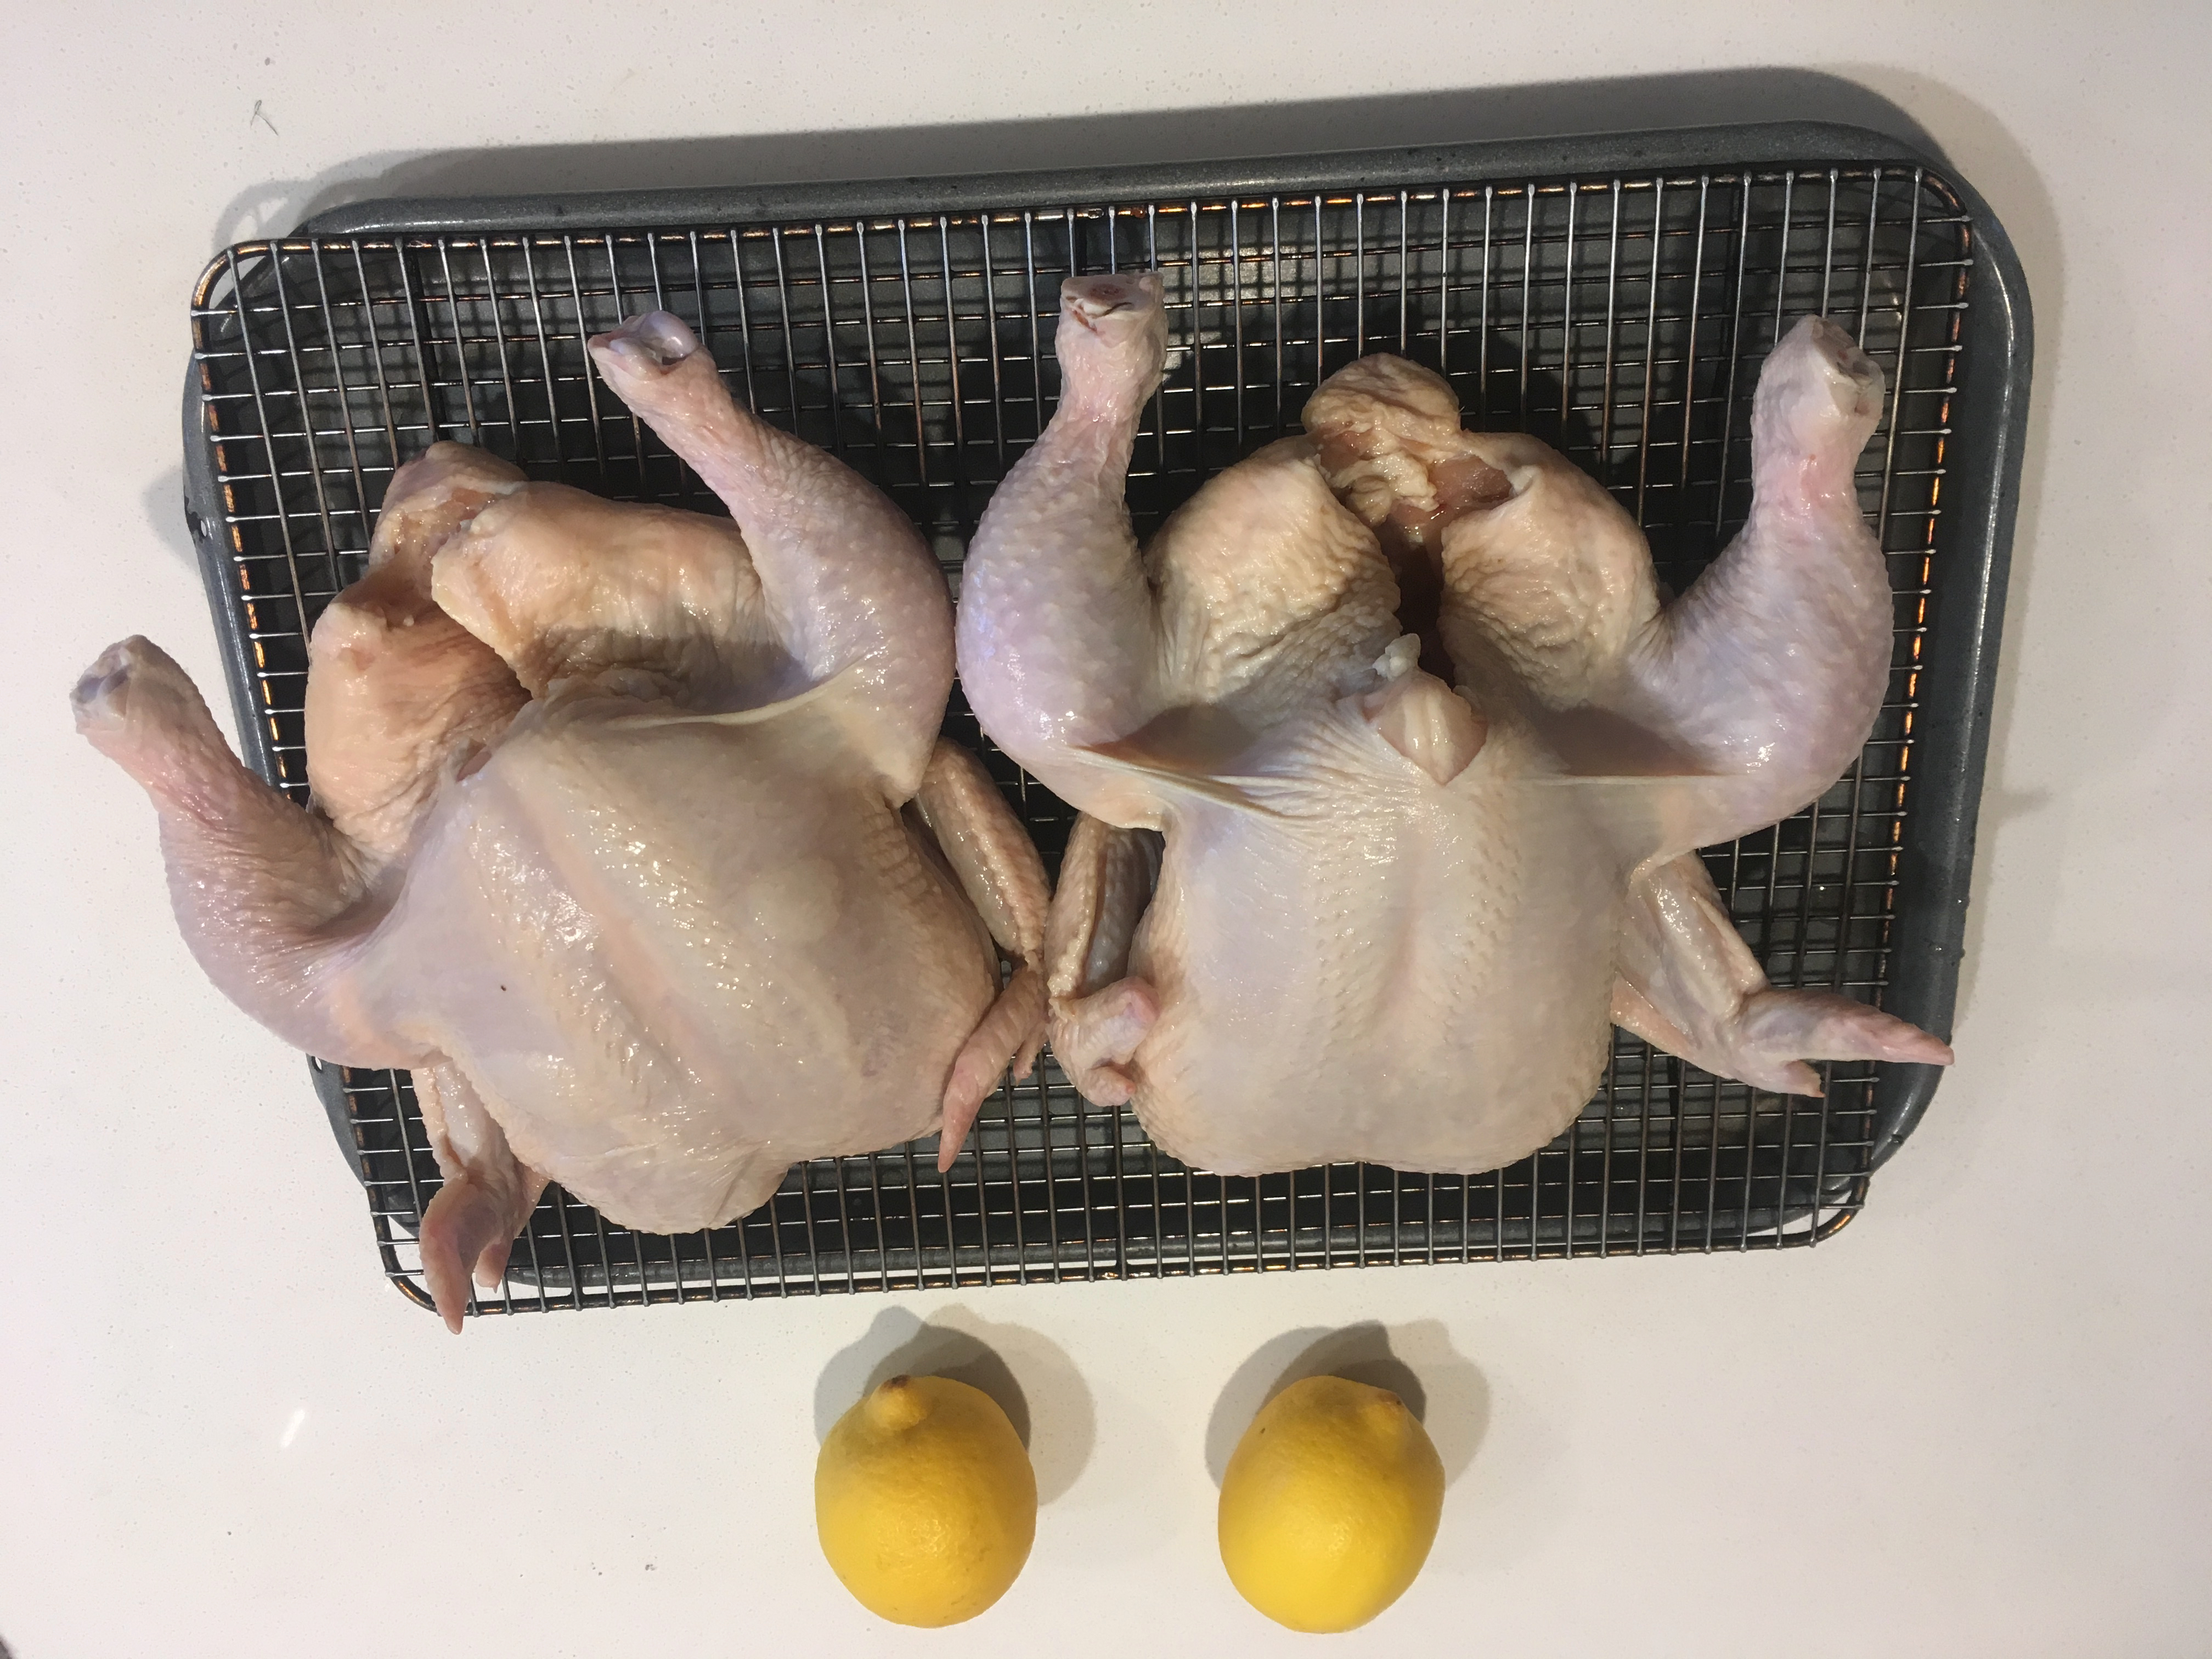
\includegraphics[width=0.25\textwidth]{\imageDir/\fileName/IMG_3197.jpg} &
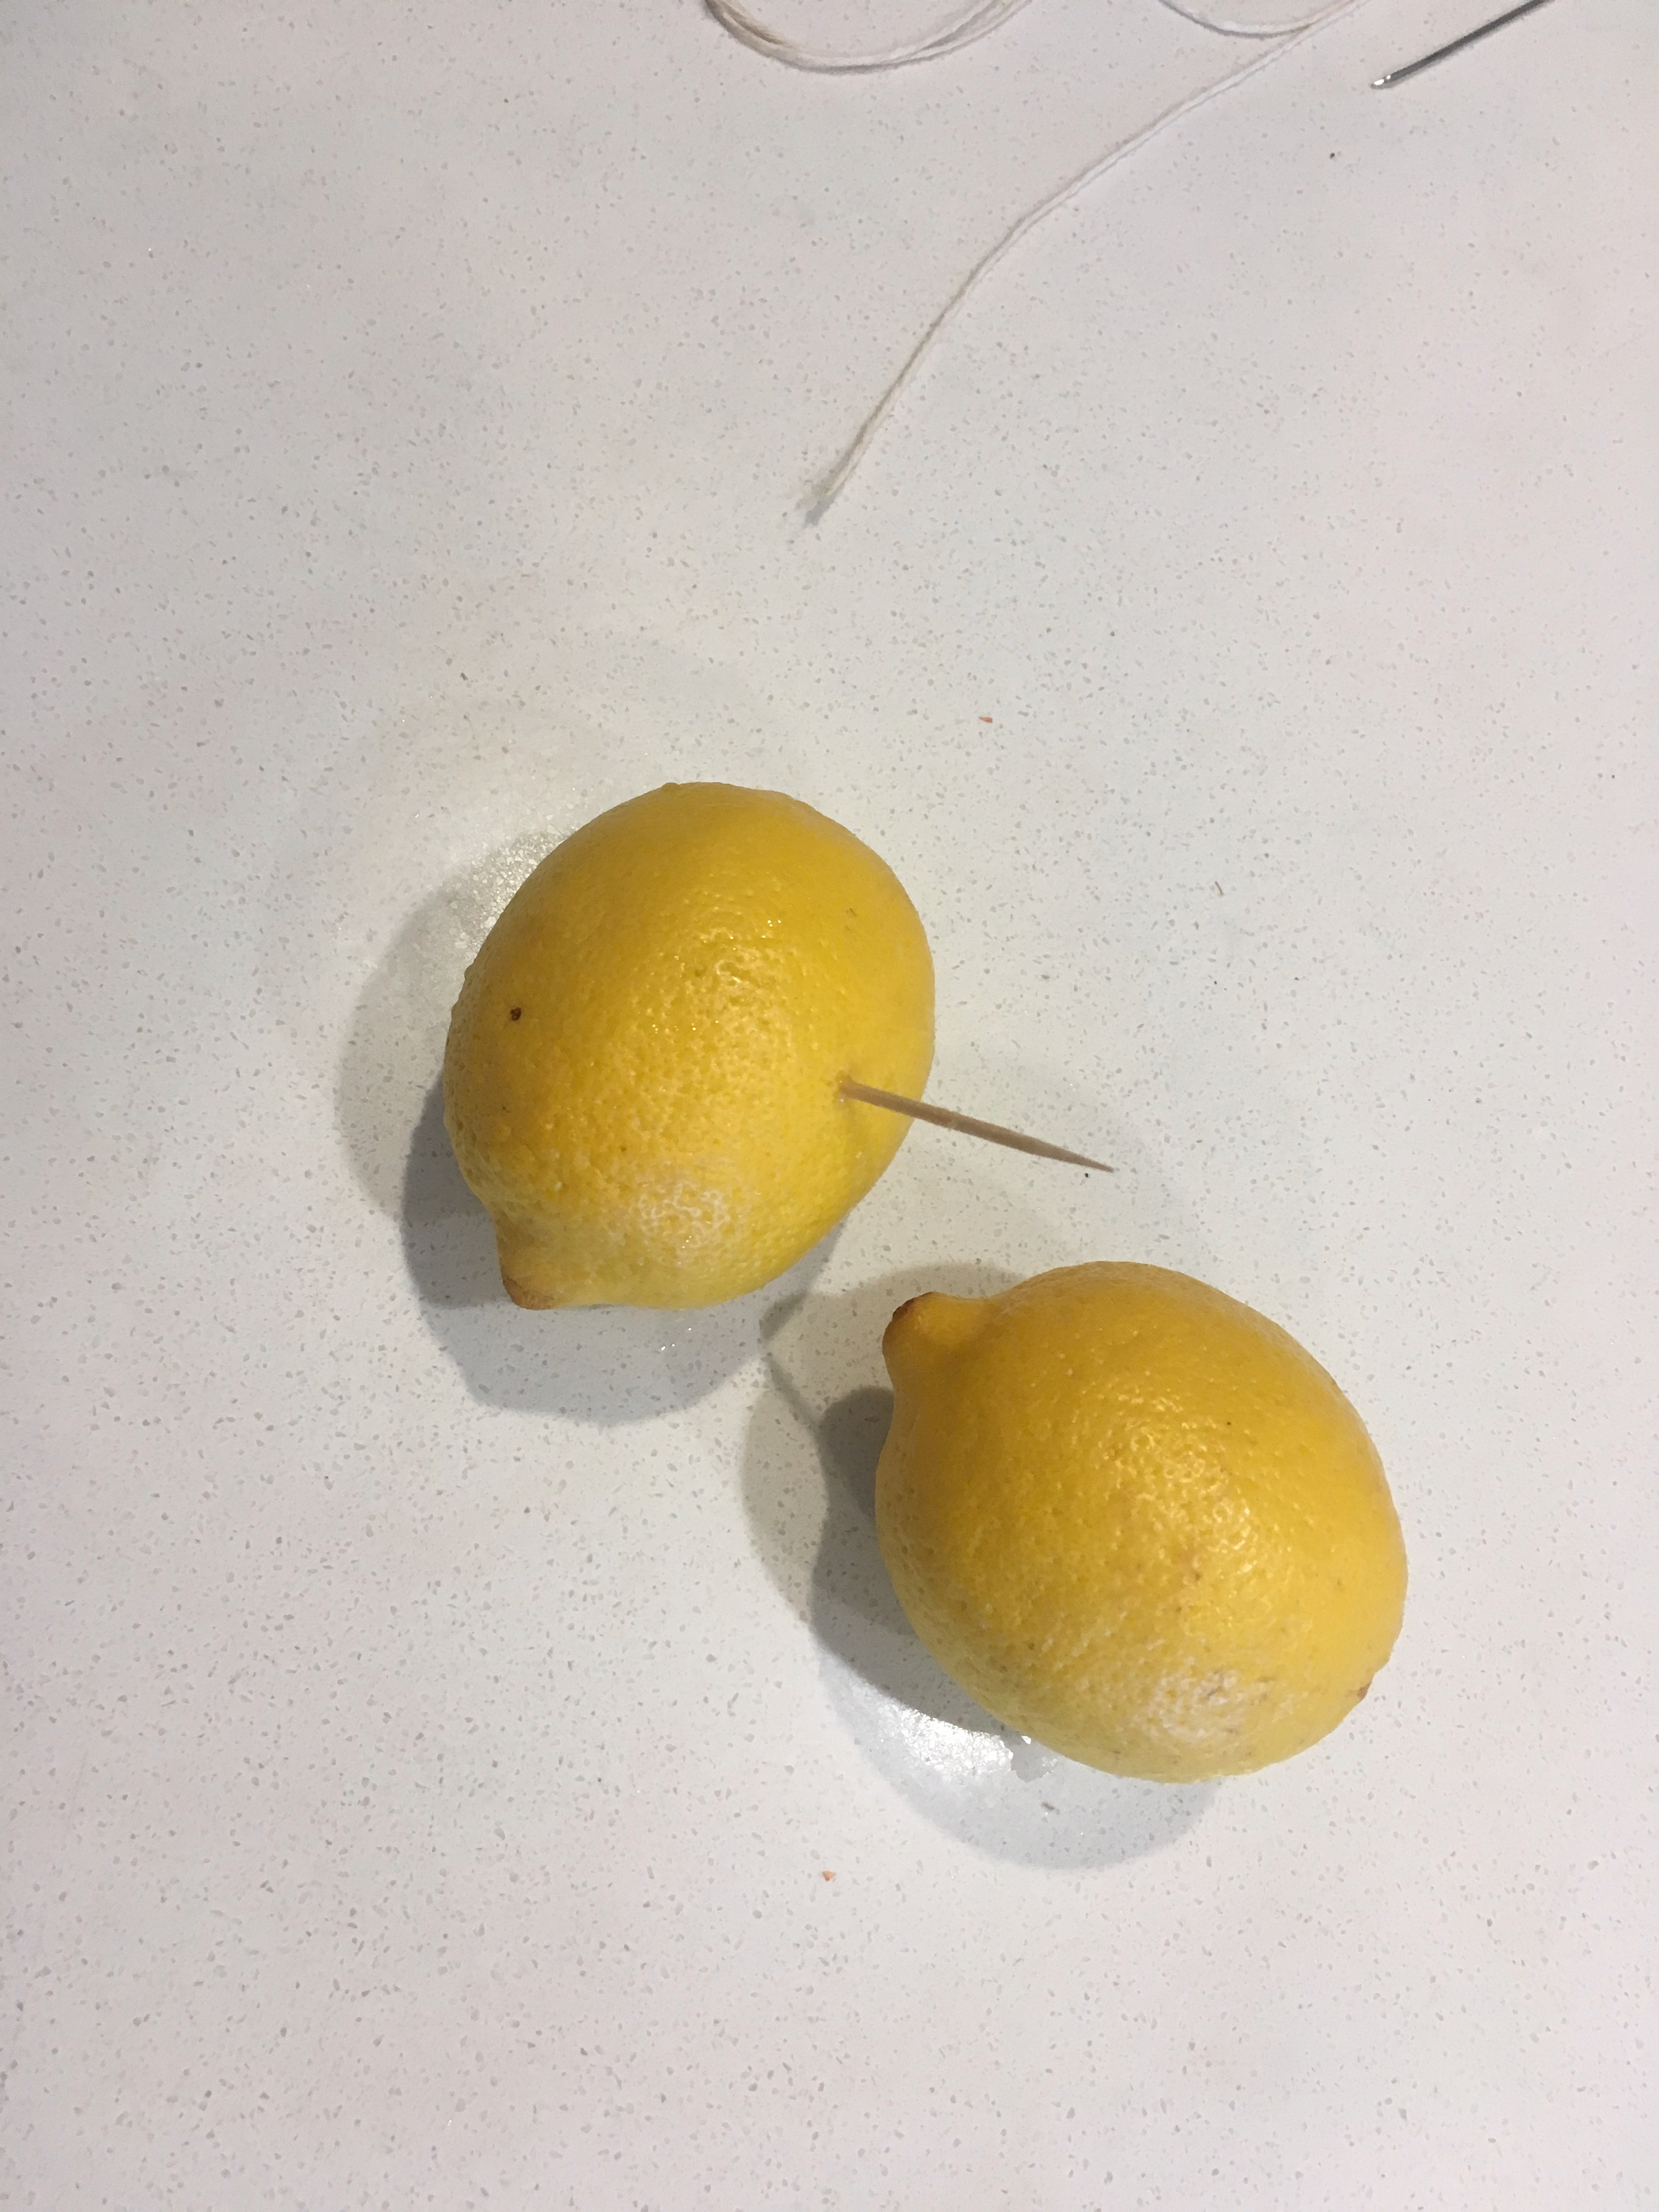
\includegraphics[width=0.25\textwidth]{\imageDir/\fileName/IMG_3212.jpg} &
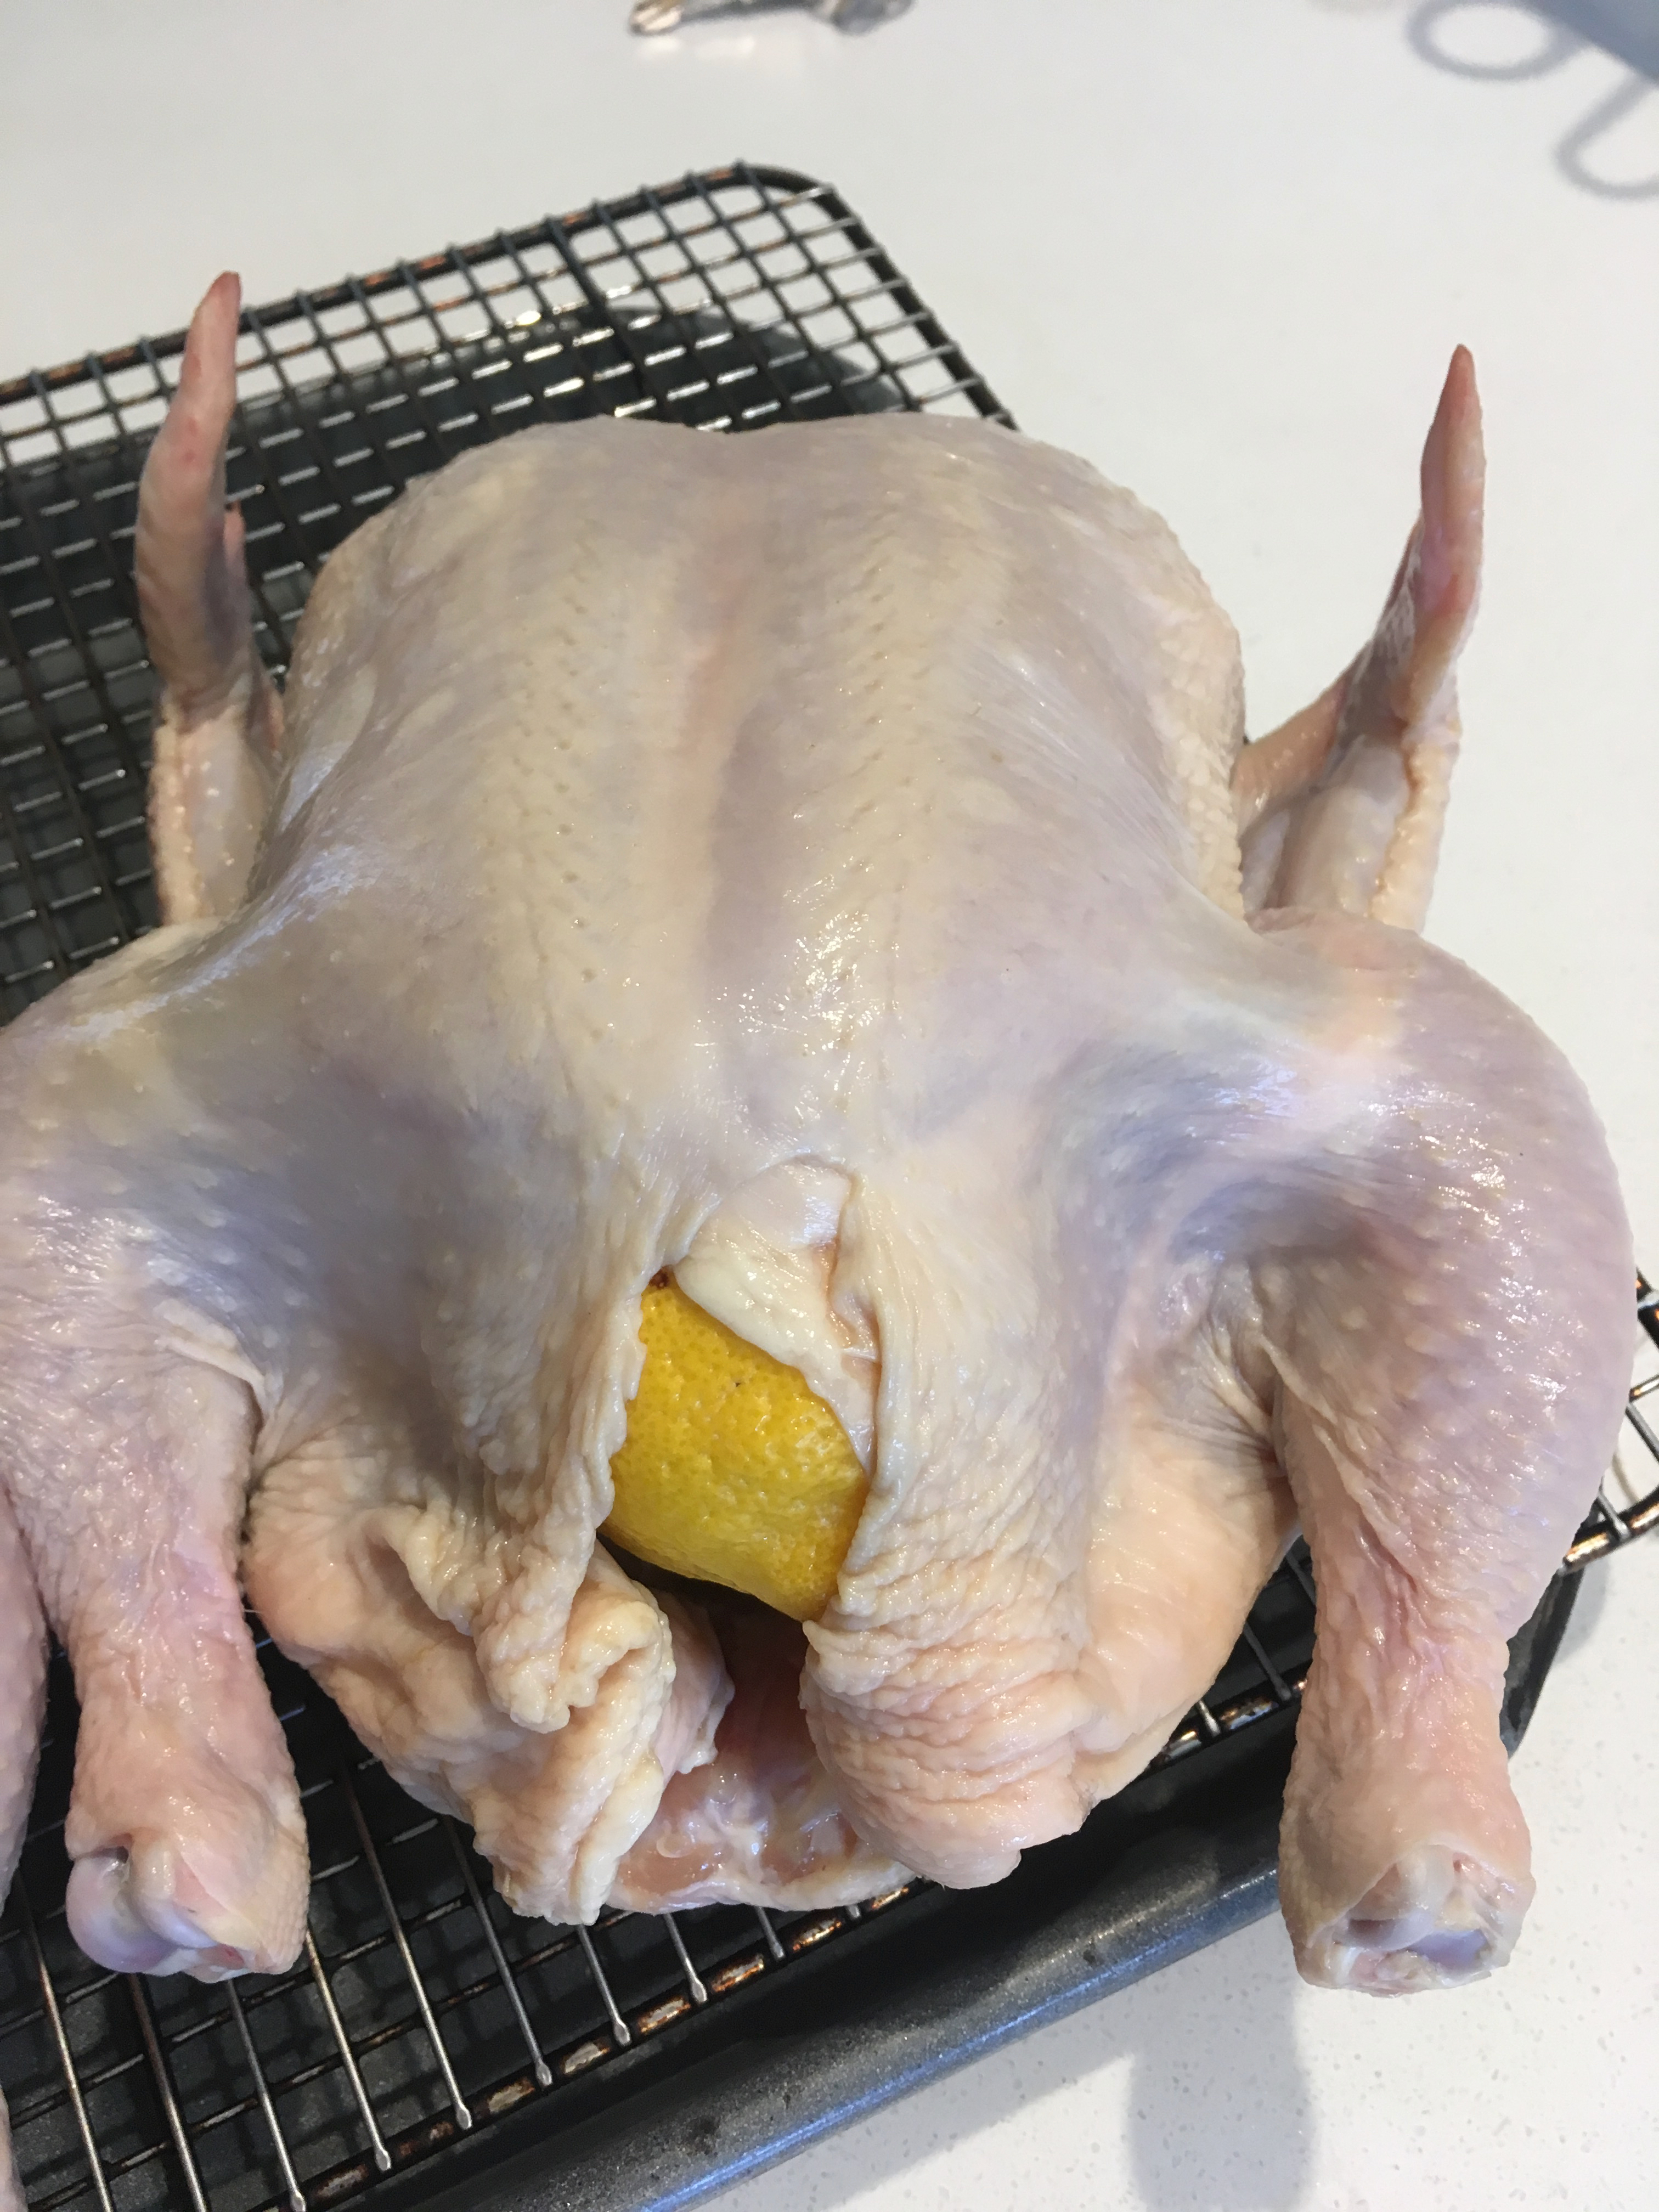
\includegraphics[width=0.25\textwidth]{\imageDir/\fileName/IMG_3213.jpg} \\
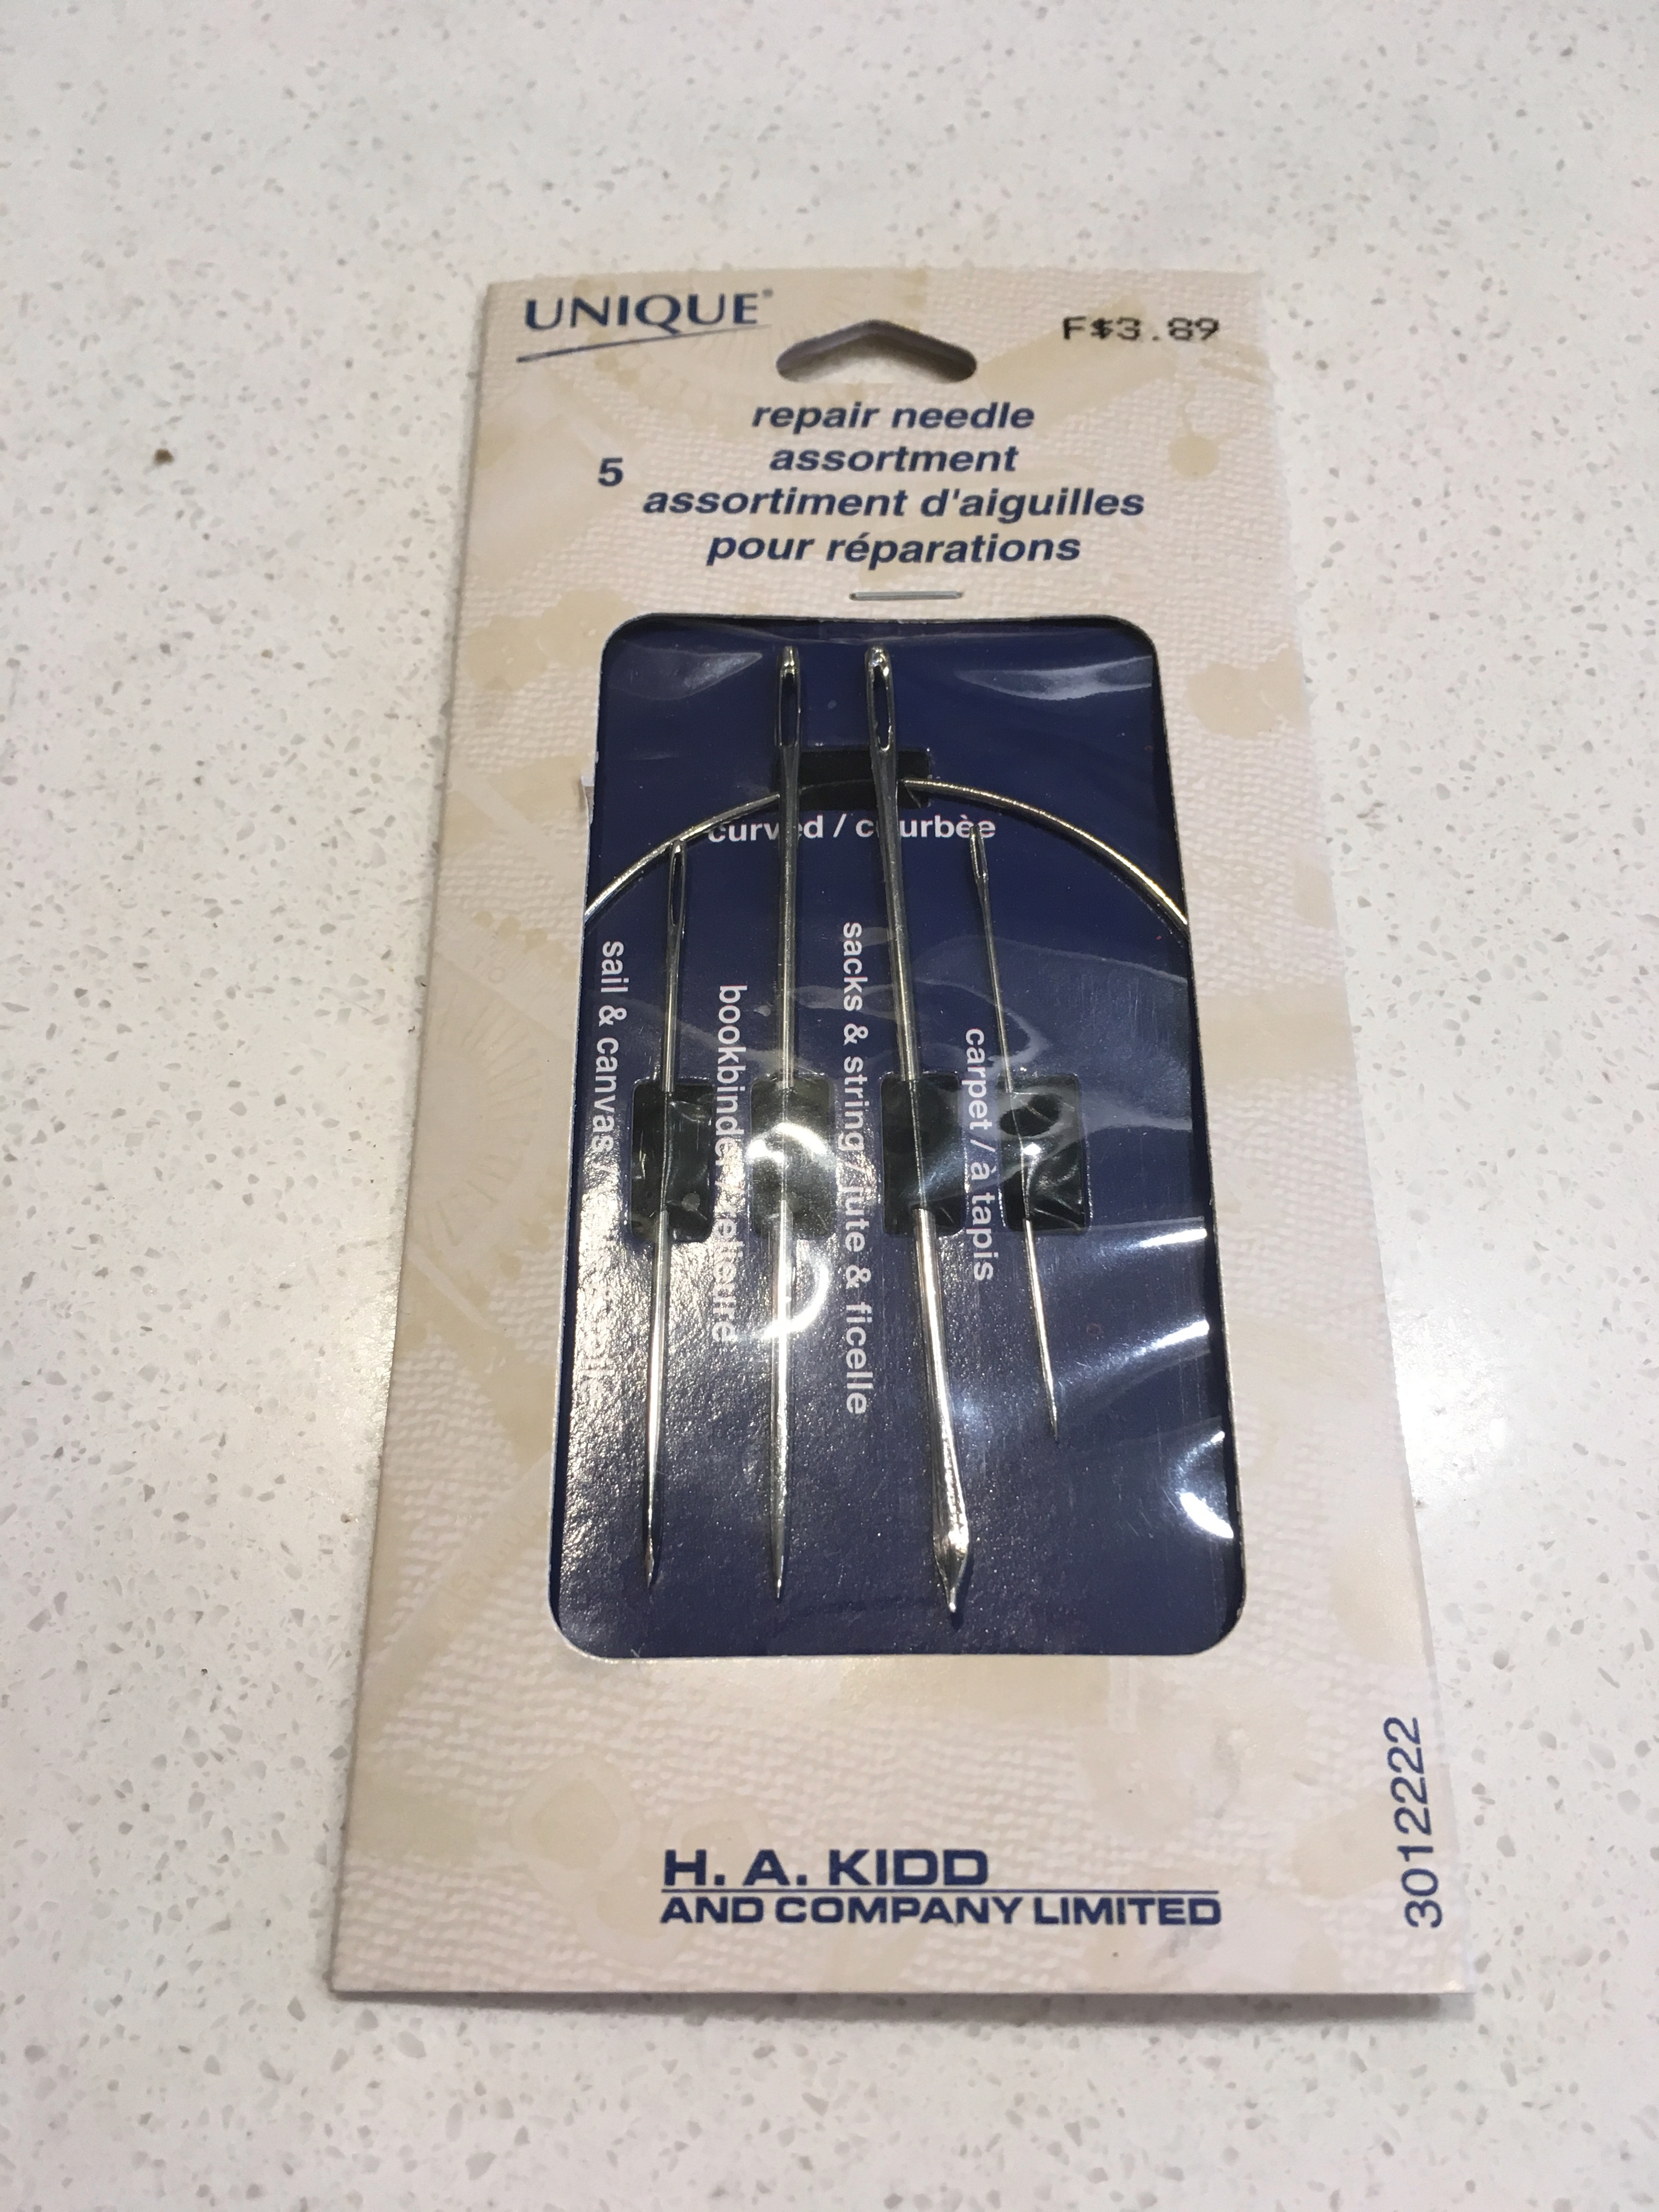
\includegraphics[width=0.25\textwidth]{\imageDir/\fileName/IMG_3206.jpg} &
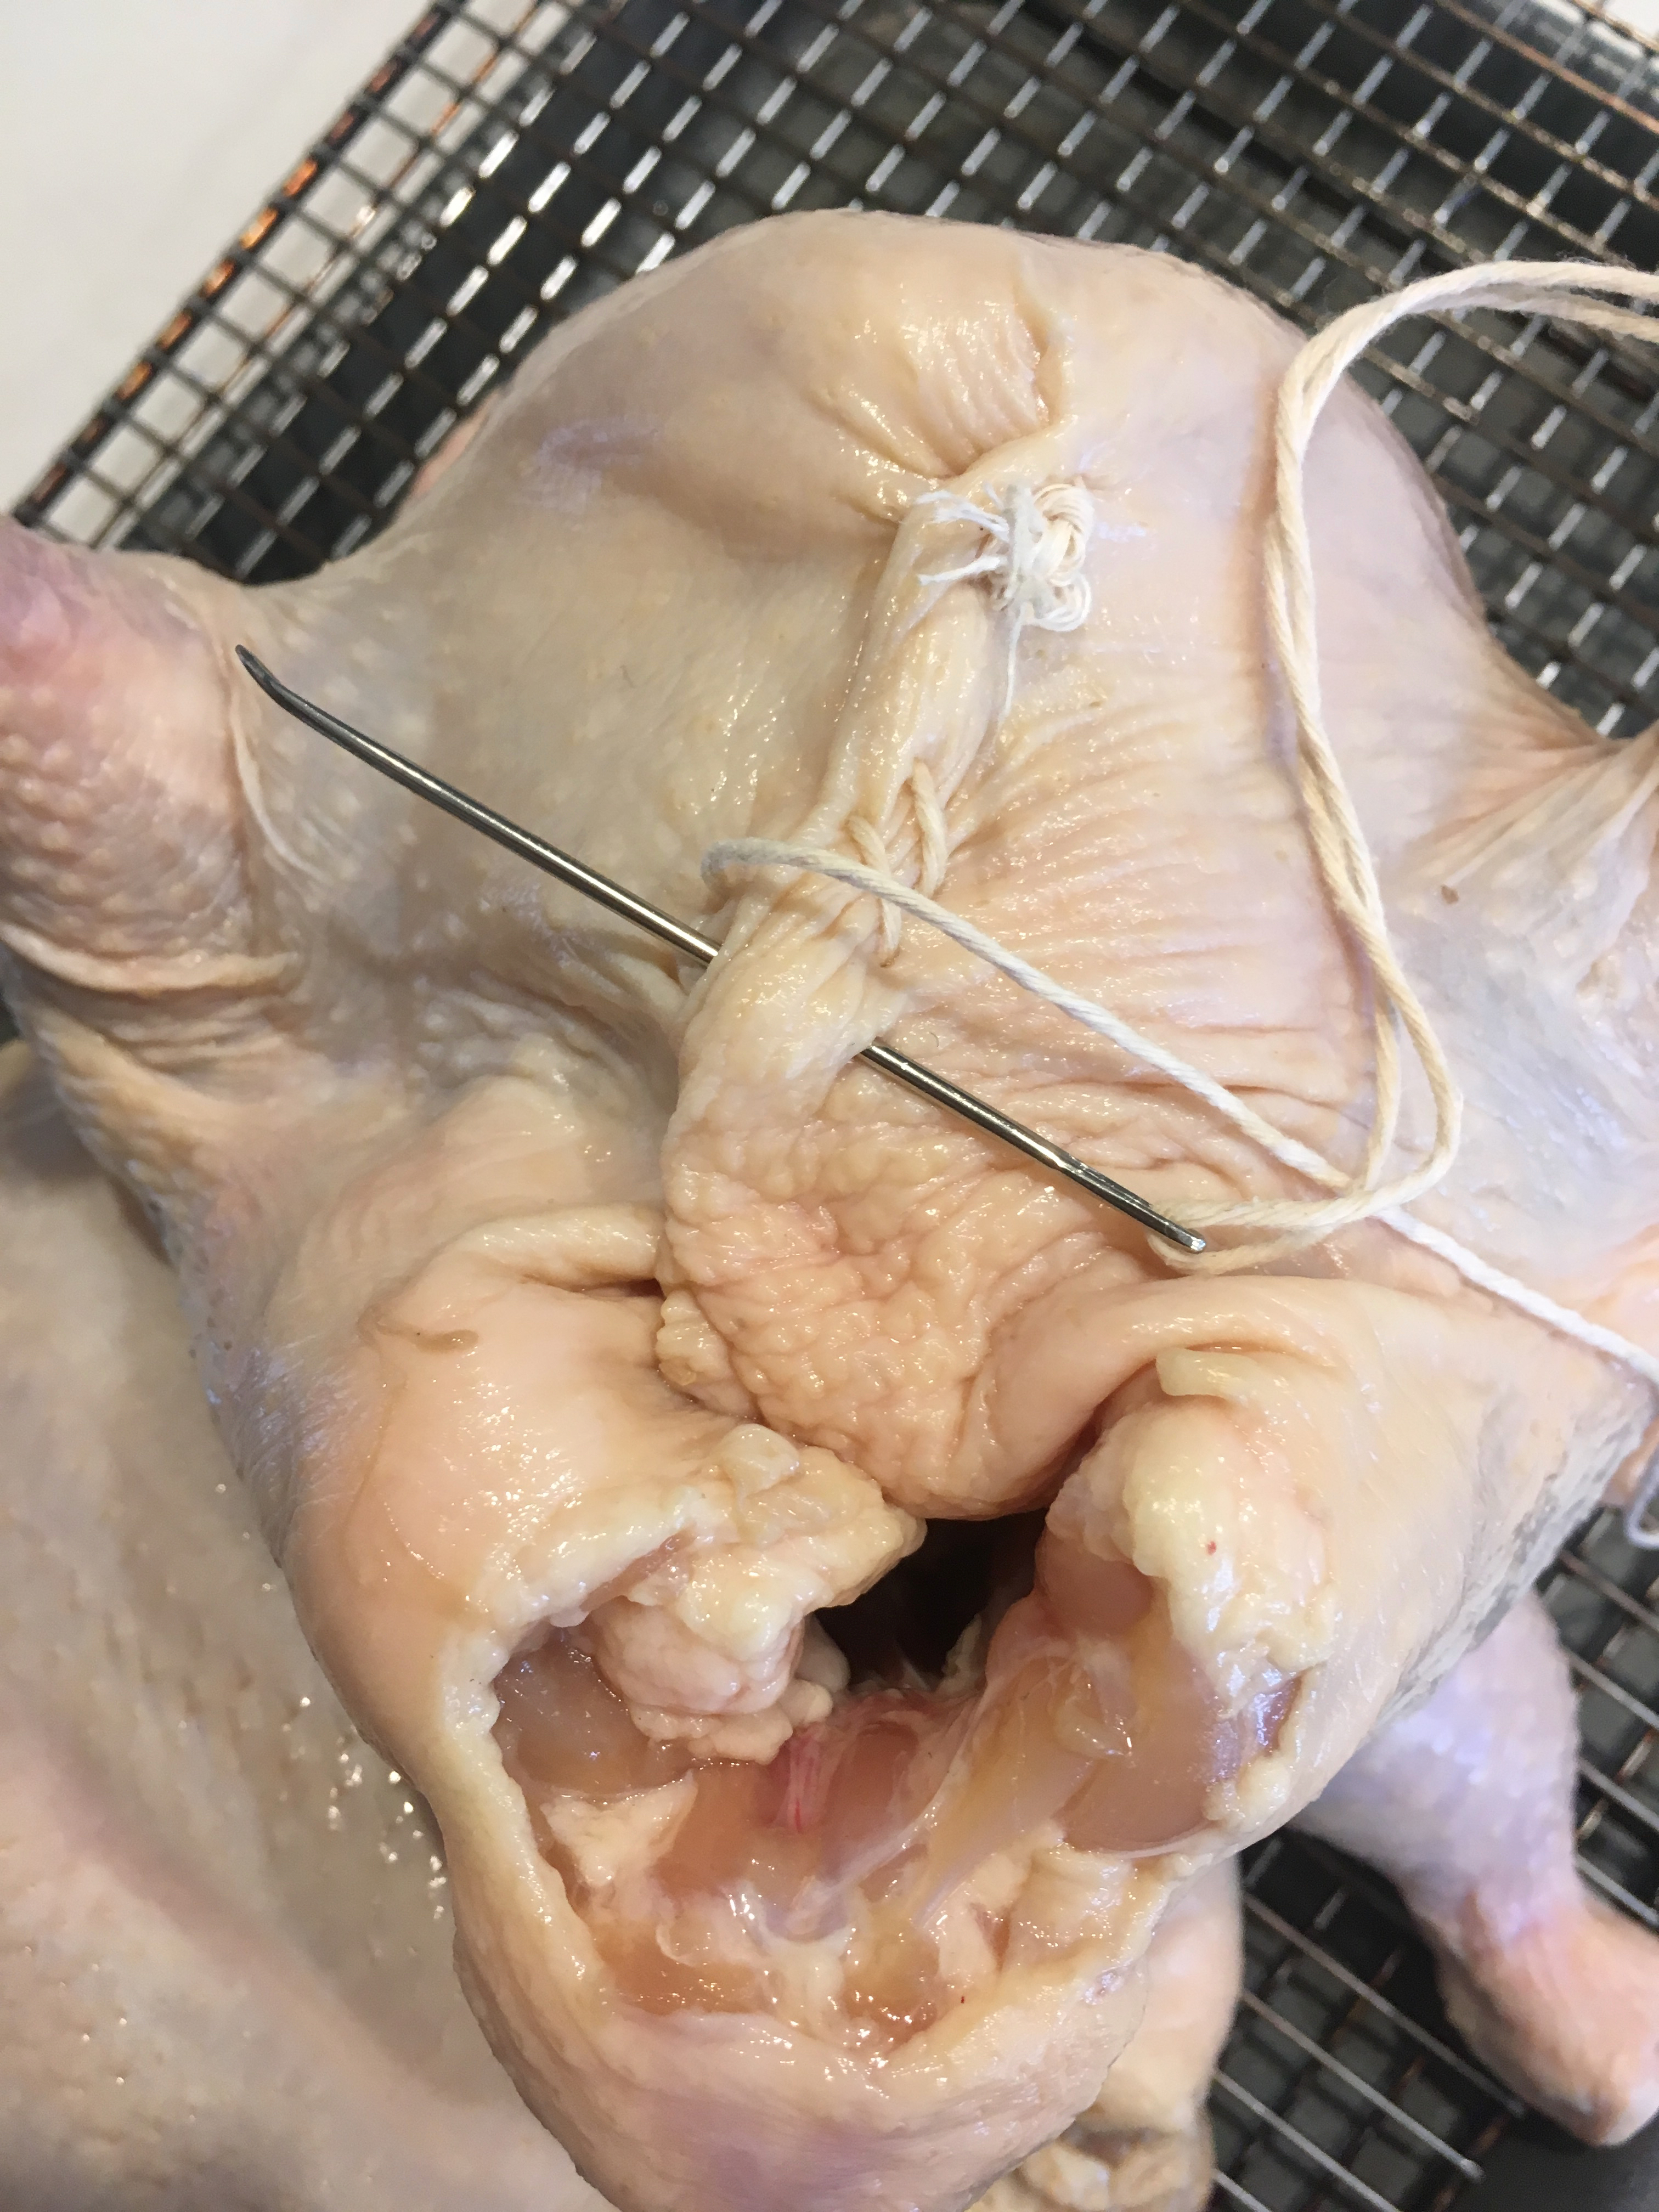
\includegraphics[width=0.25\textwidth]{\imageDir/\fileName/IMG_3214.jpg} &
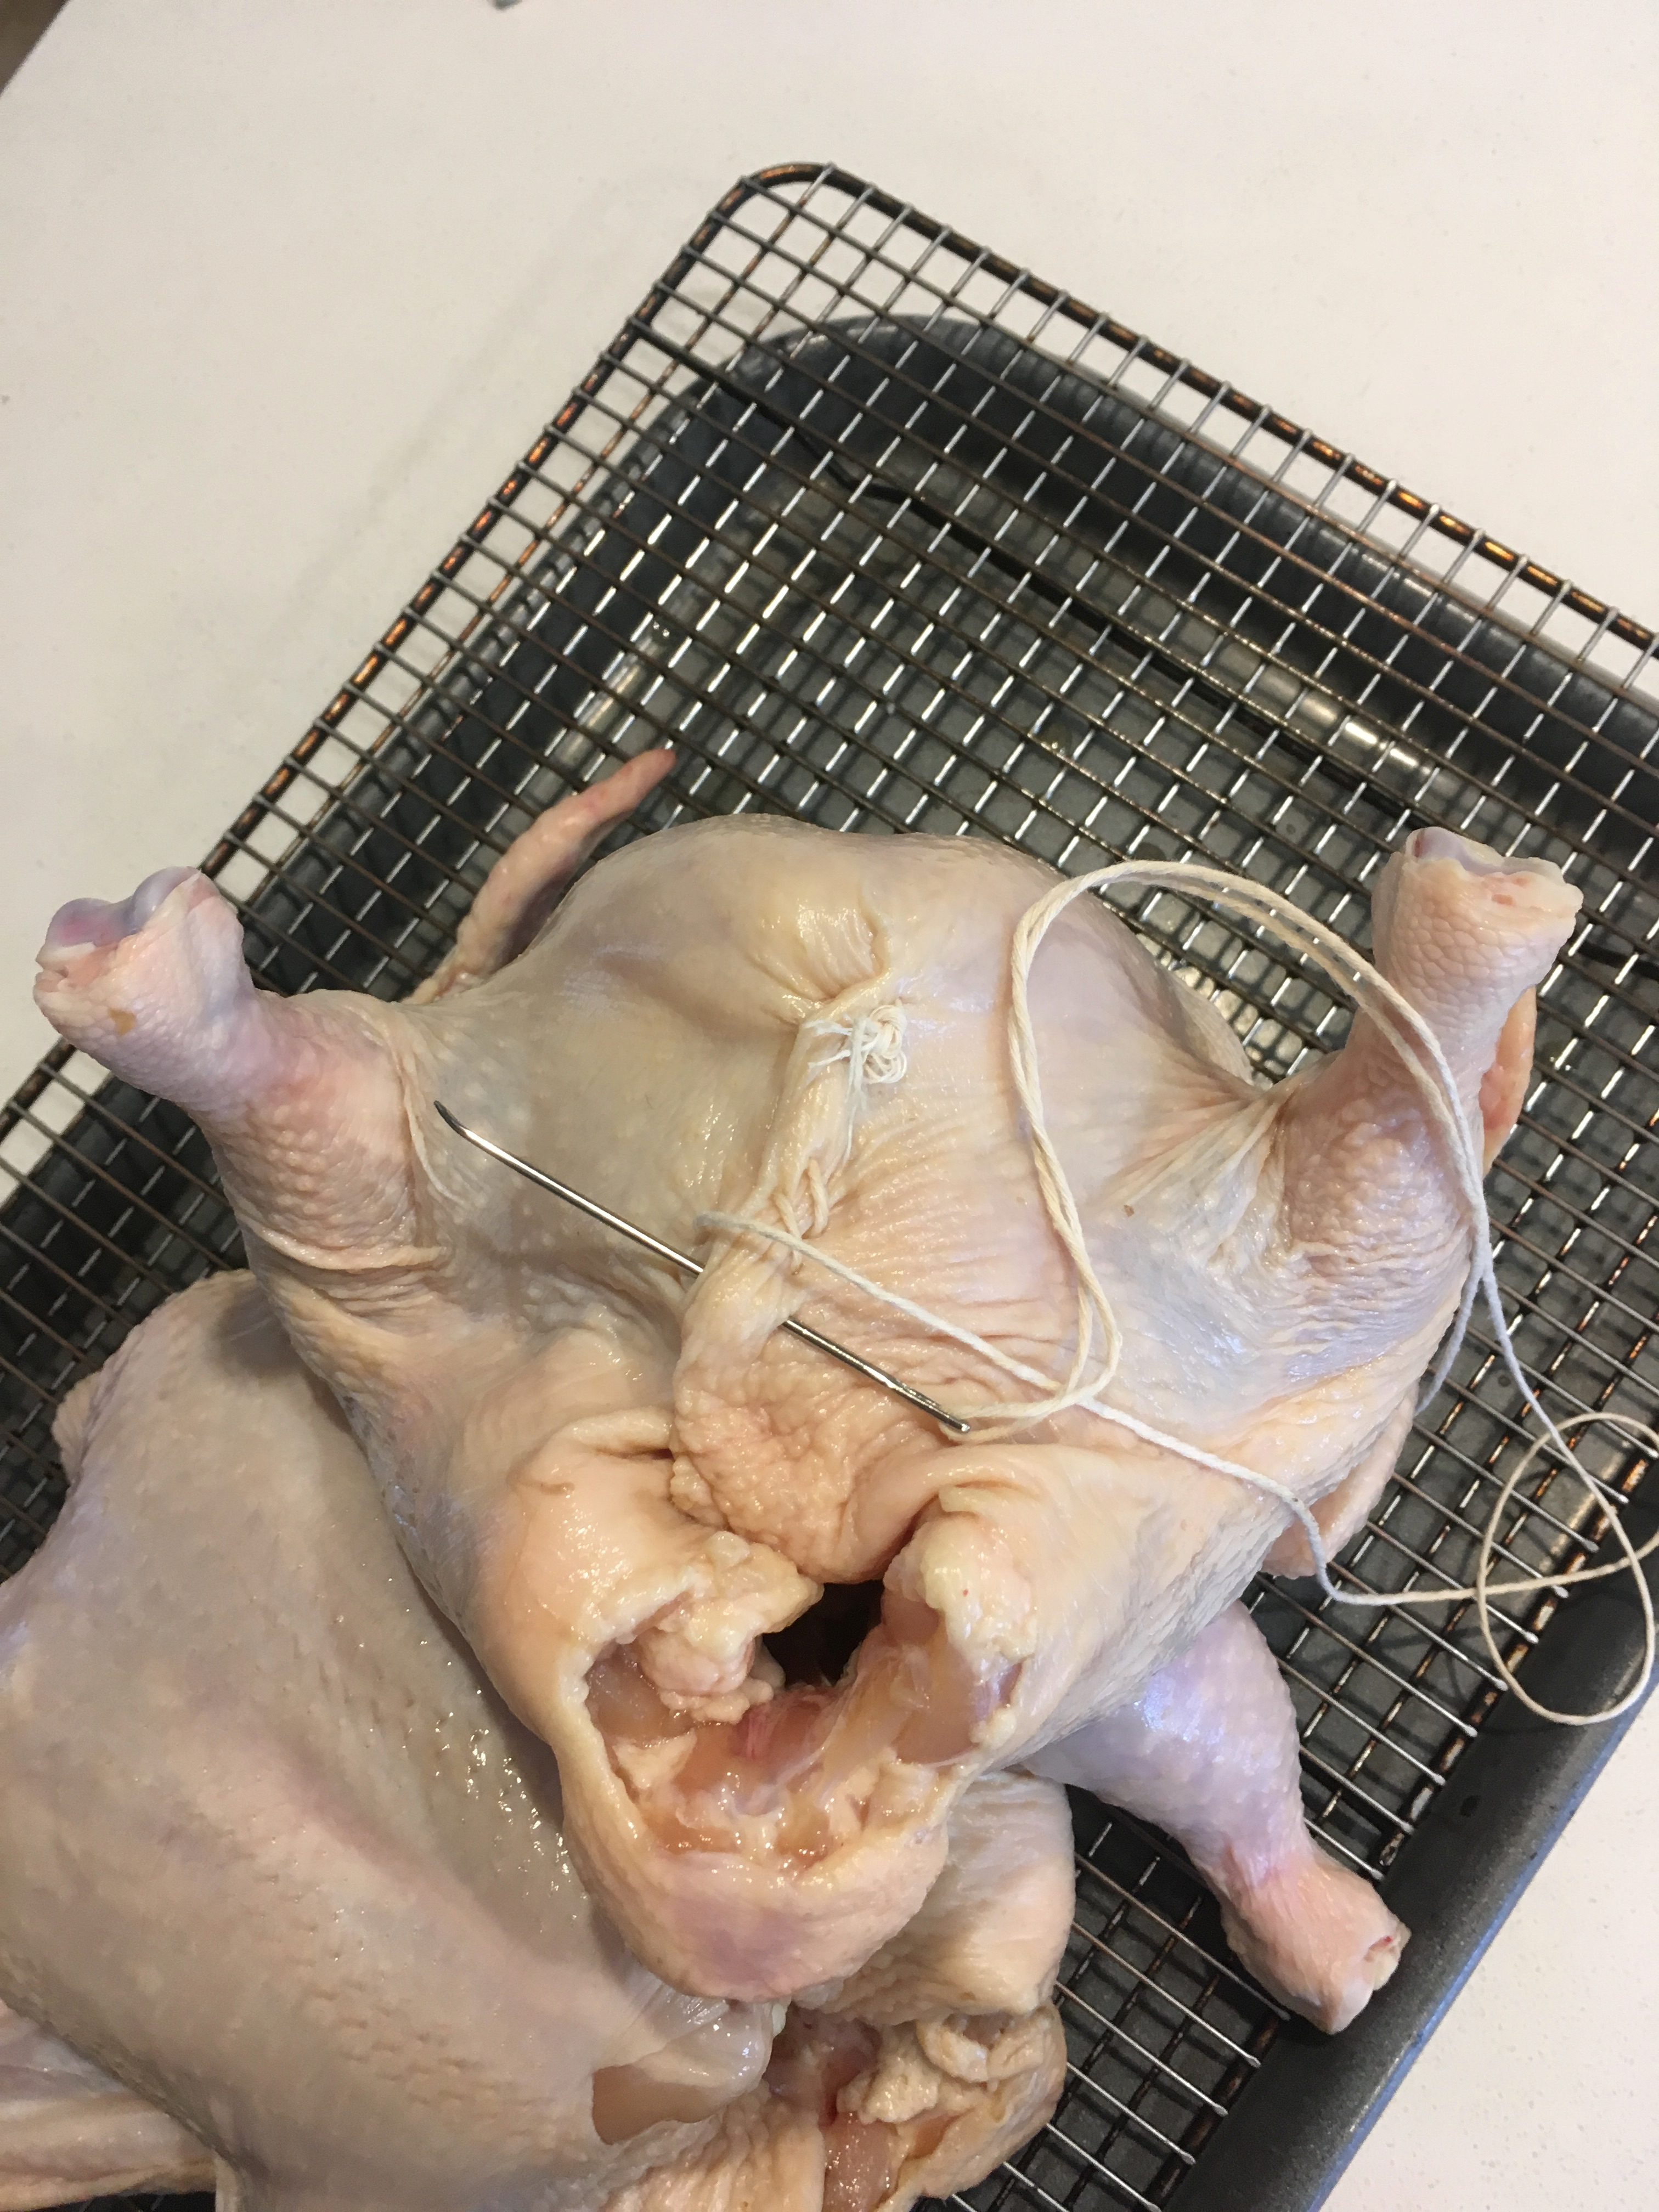
\includegraphics[width=0.25\textwidth]{\imageDir/\fileName/IMG_3216.jpg} \\
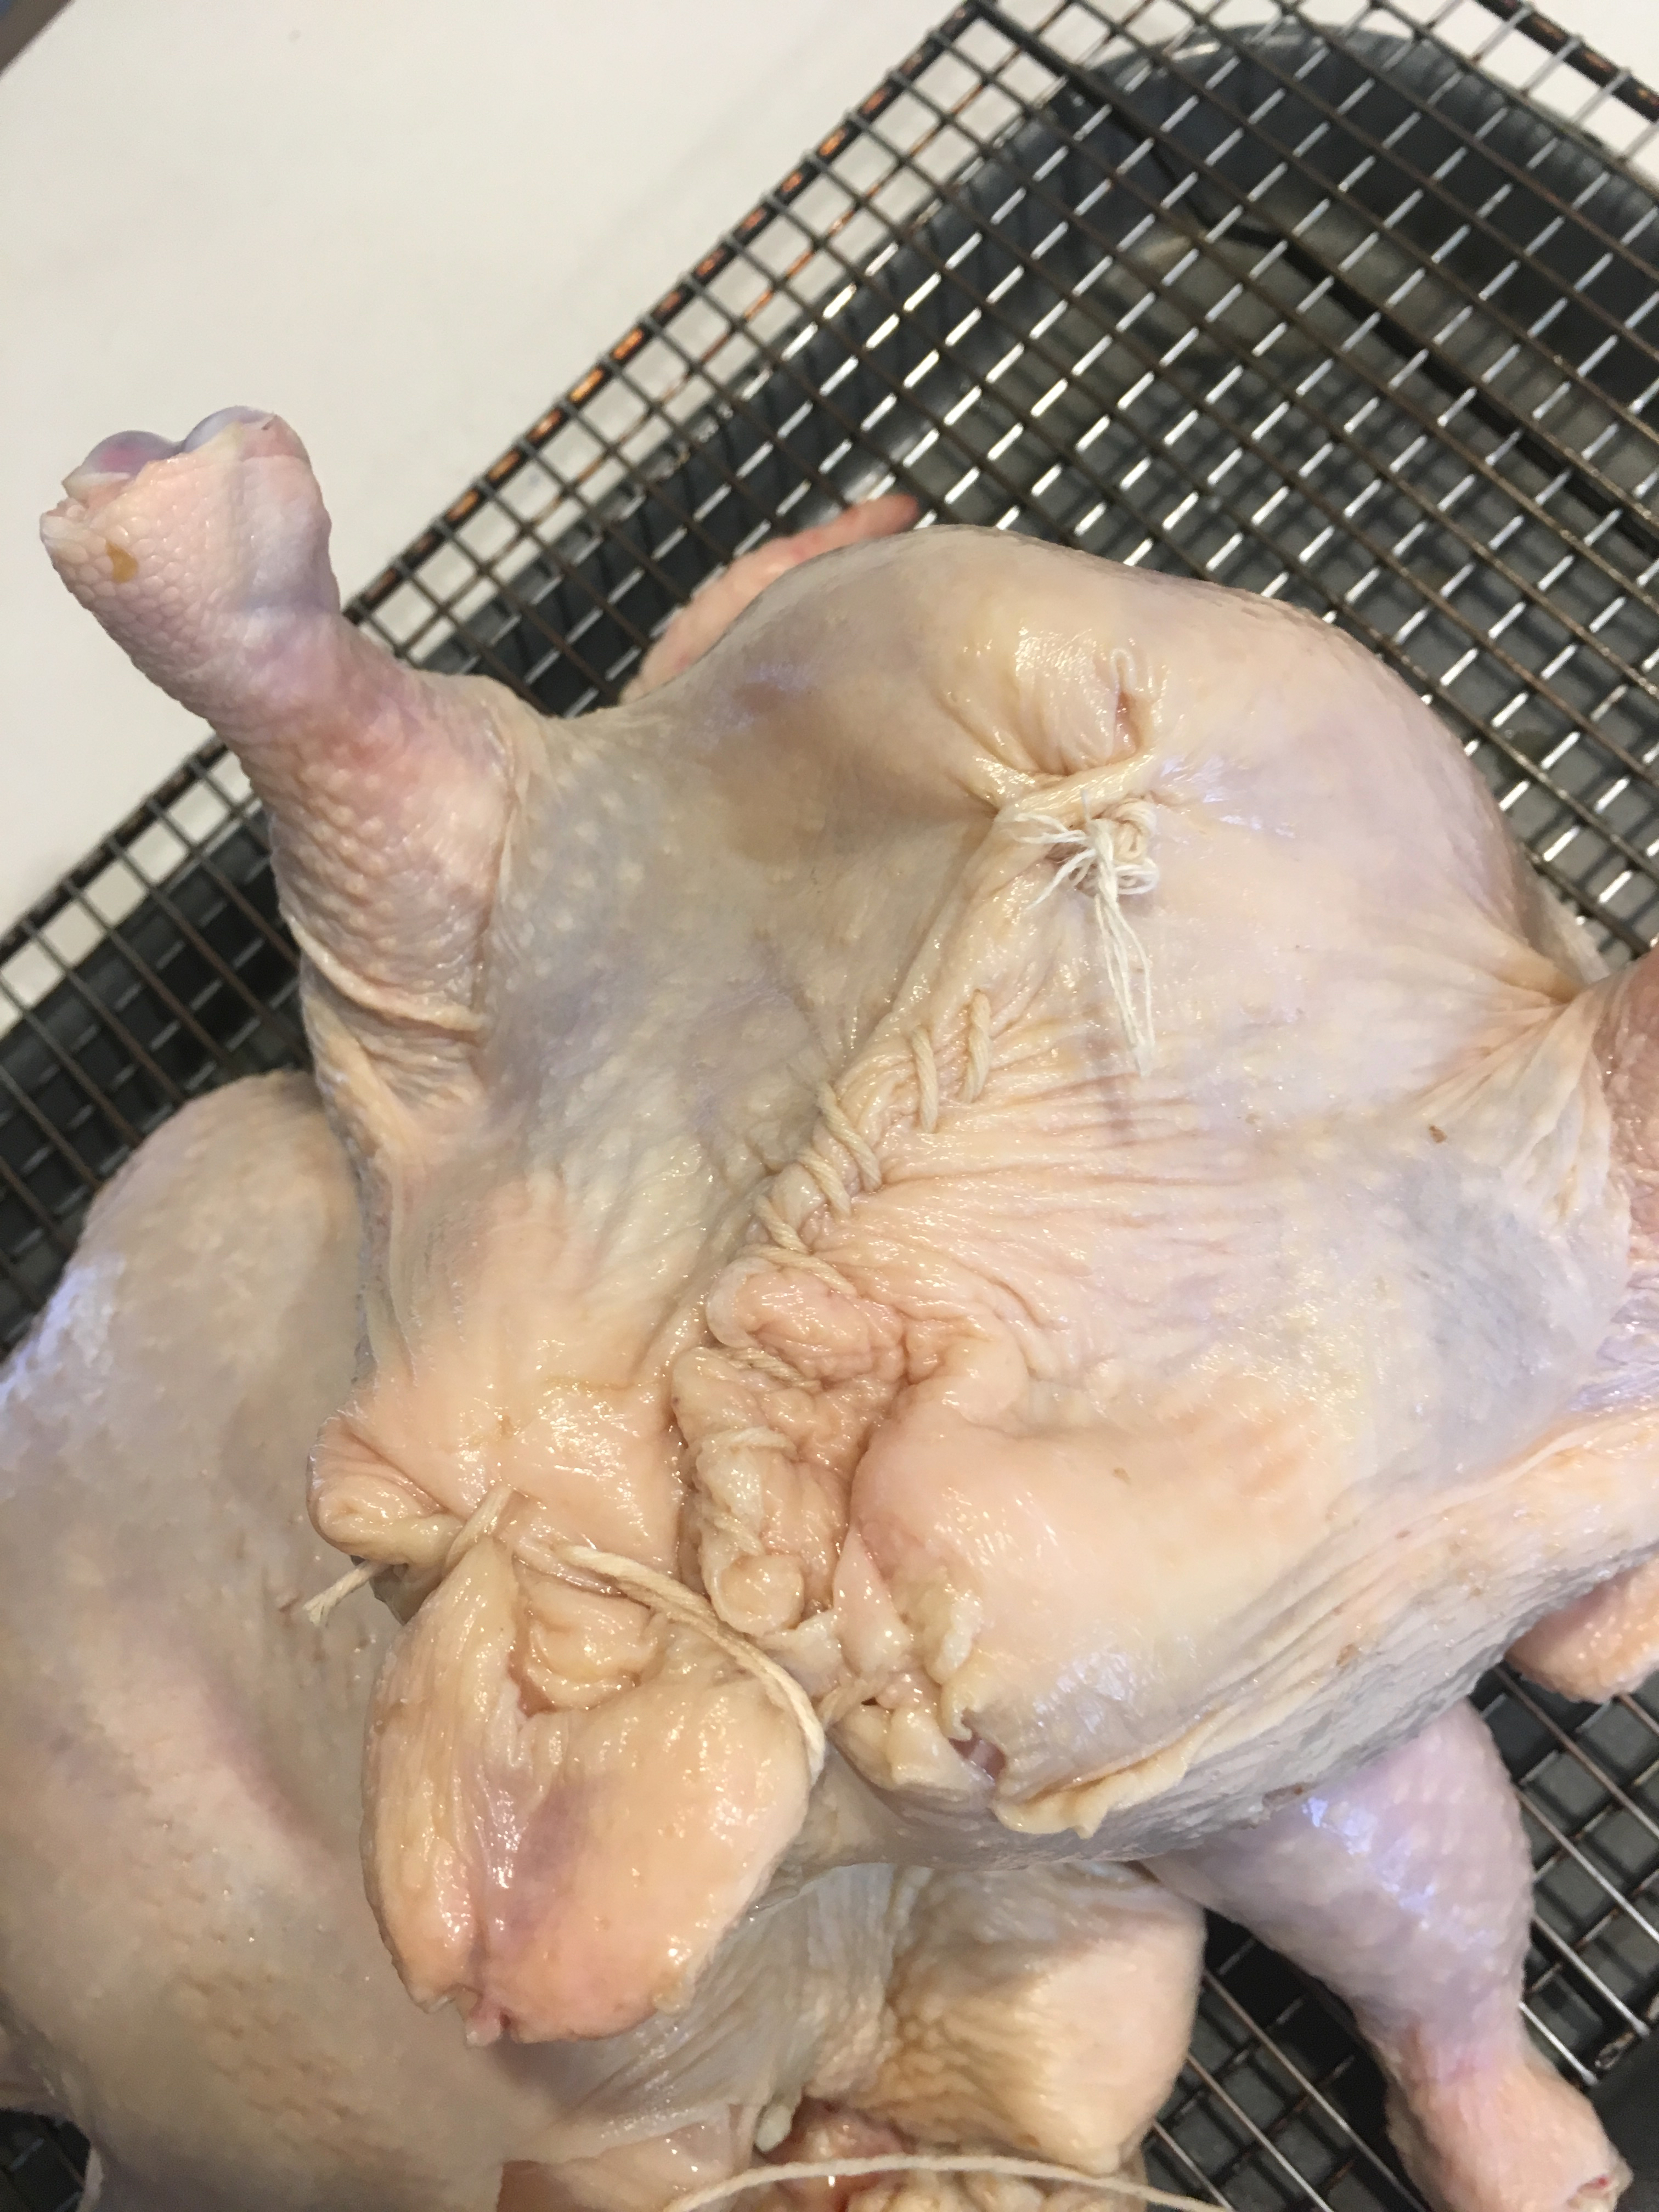
\includegraphics[width=0.25\textwidth]{\imageDir/\fileName/IMG_3217.jpg} &
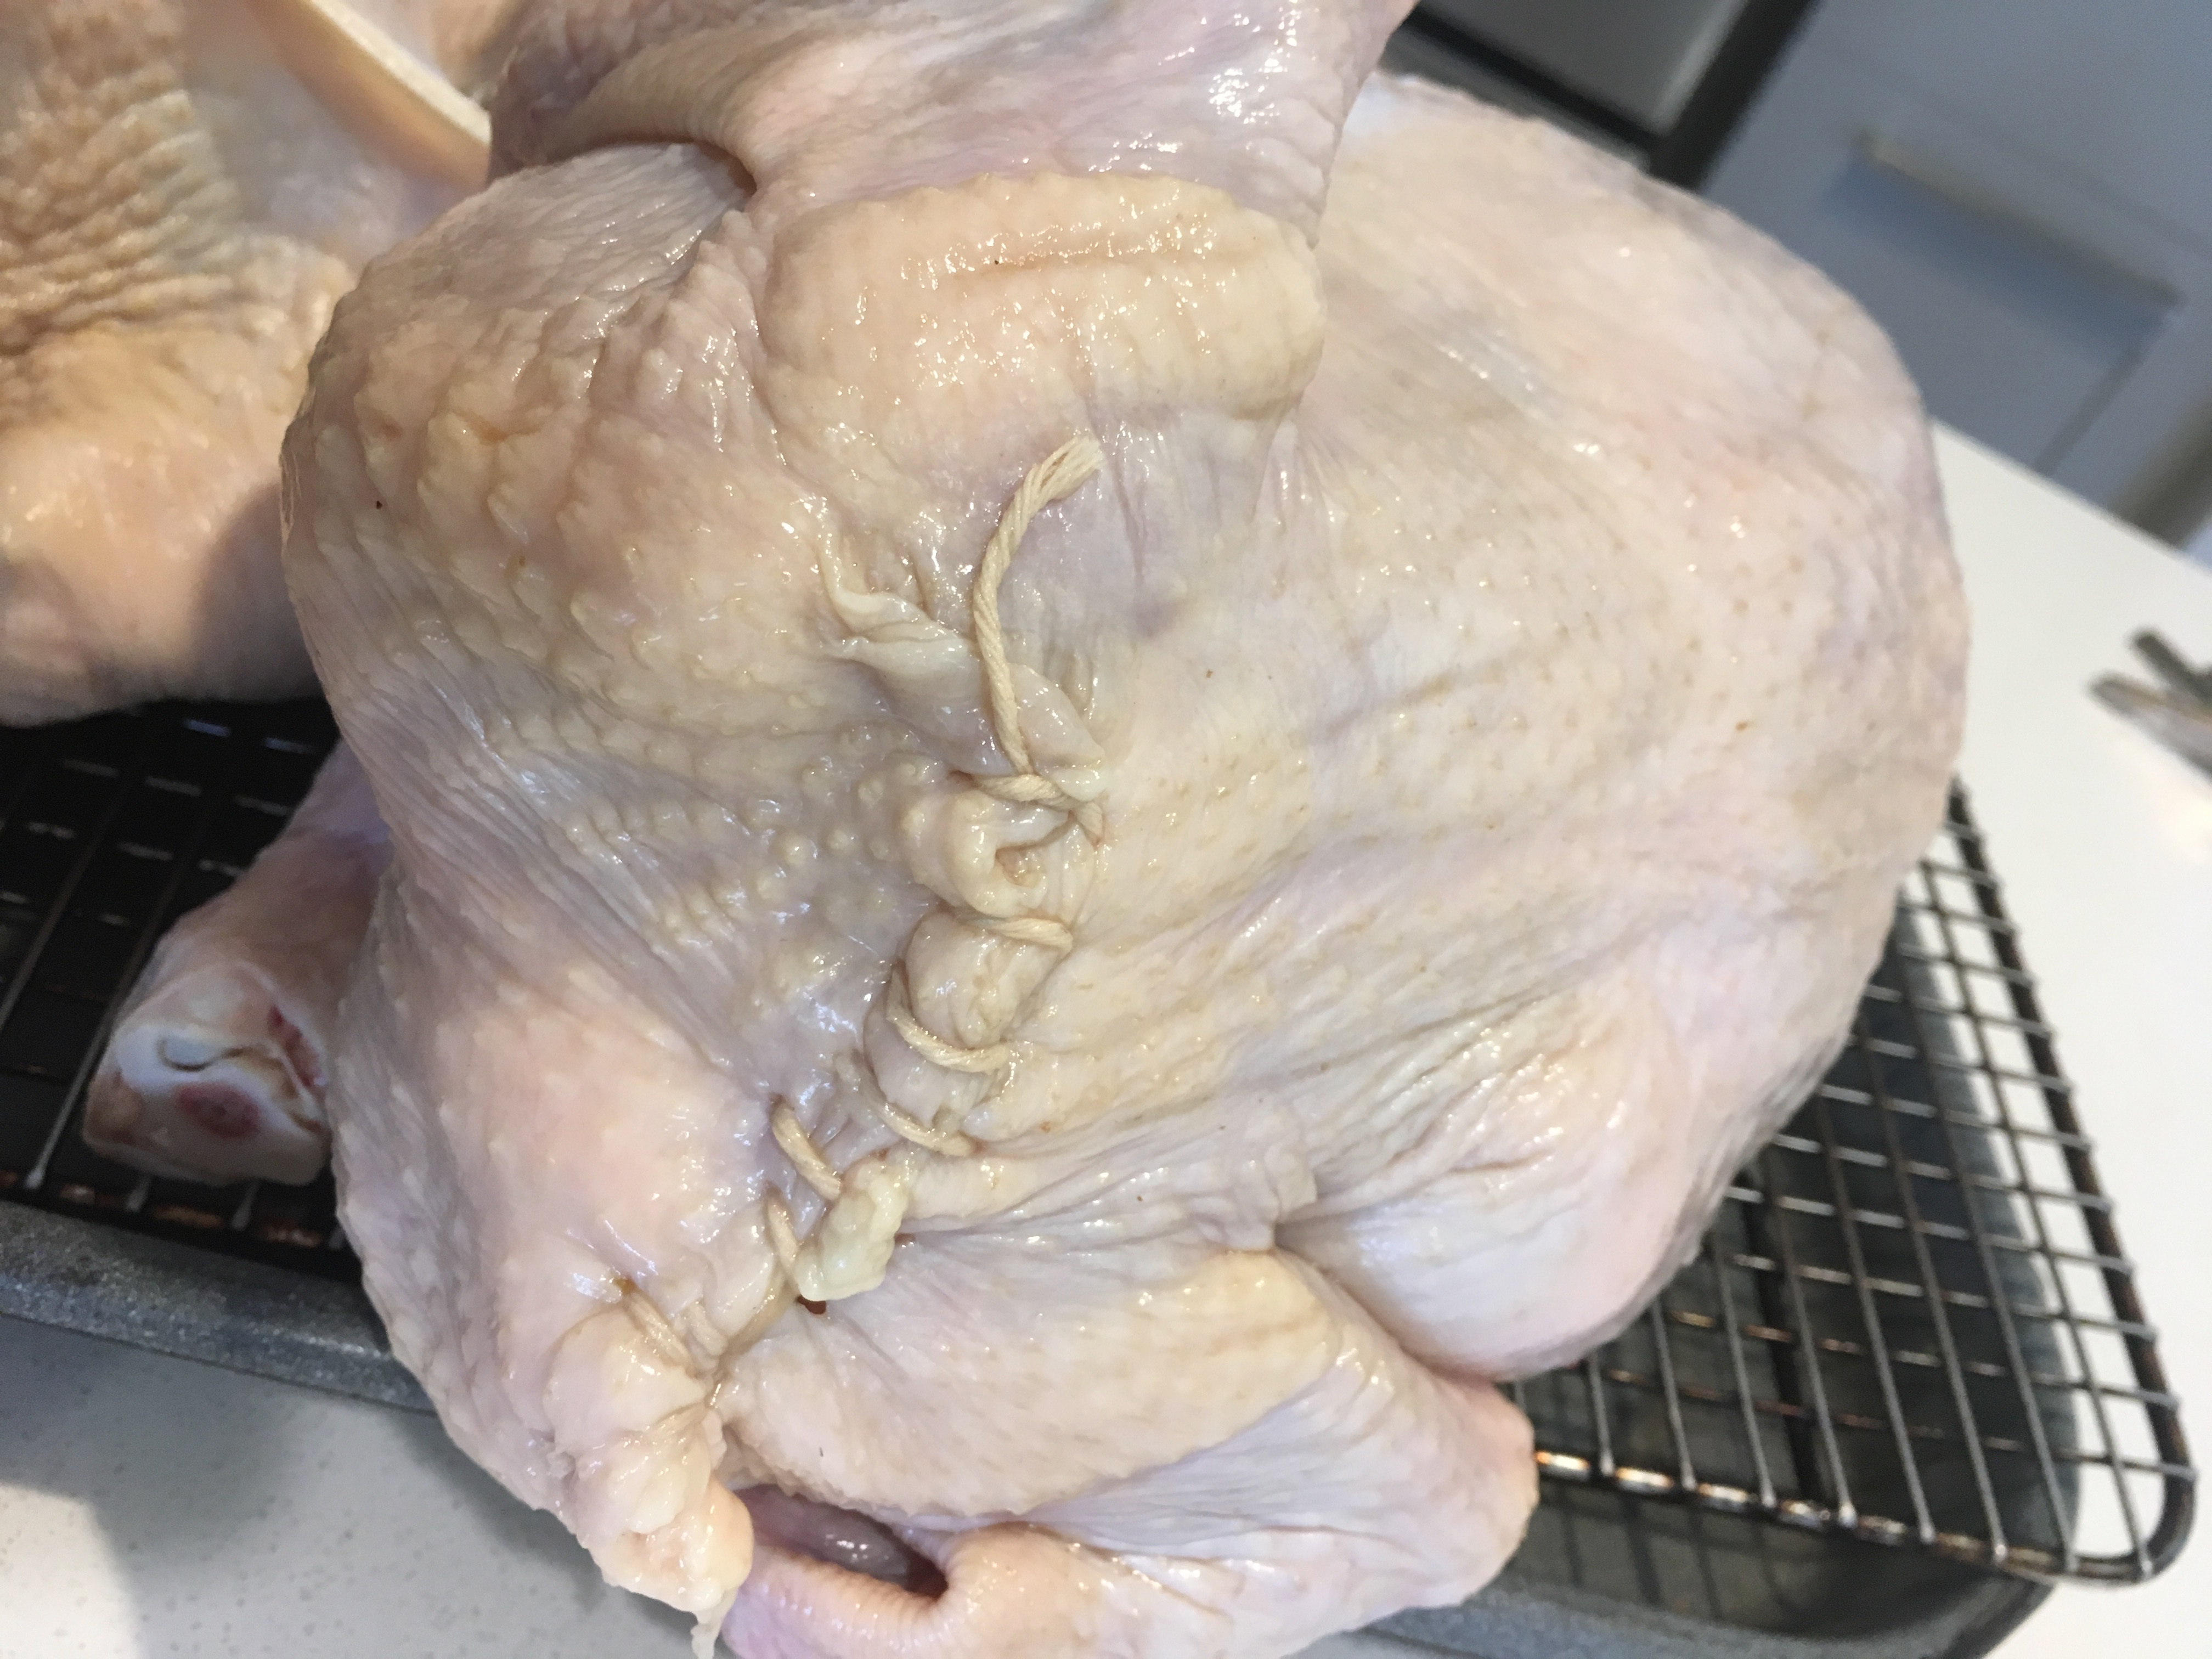
\includegraphics[width=0.25\textwidth]{\imageDir/\fileName/IMG_3218.jpg} &
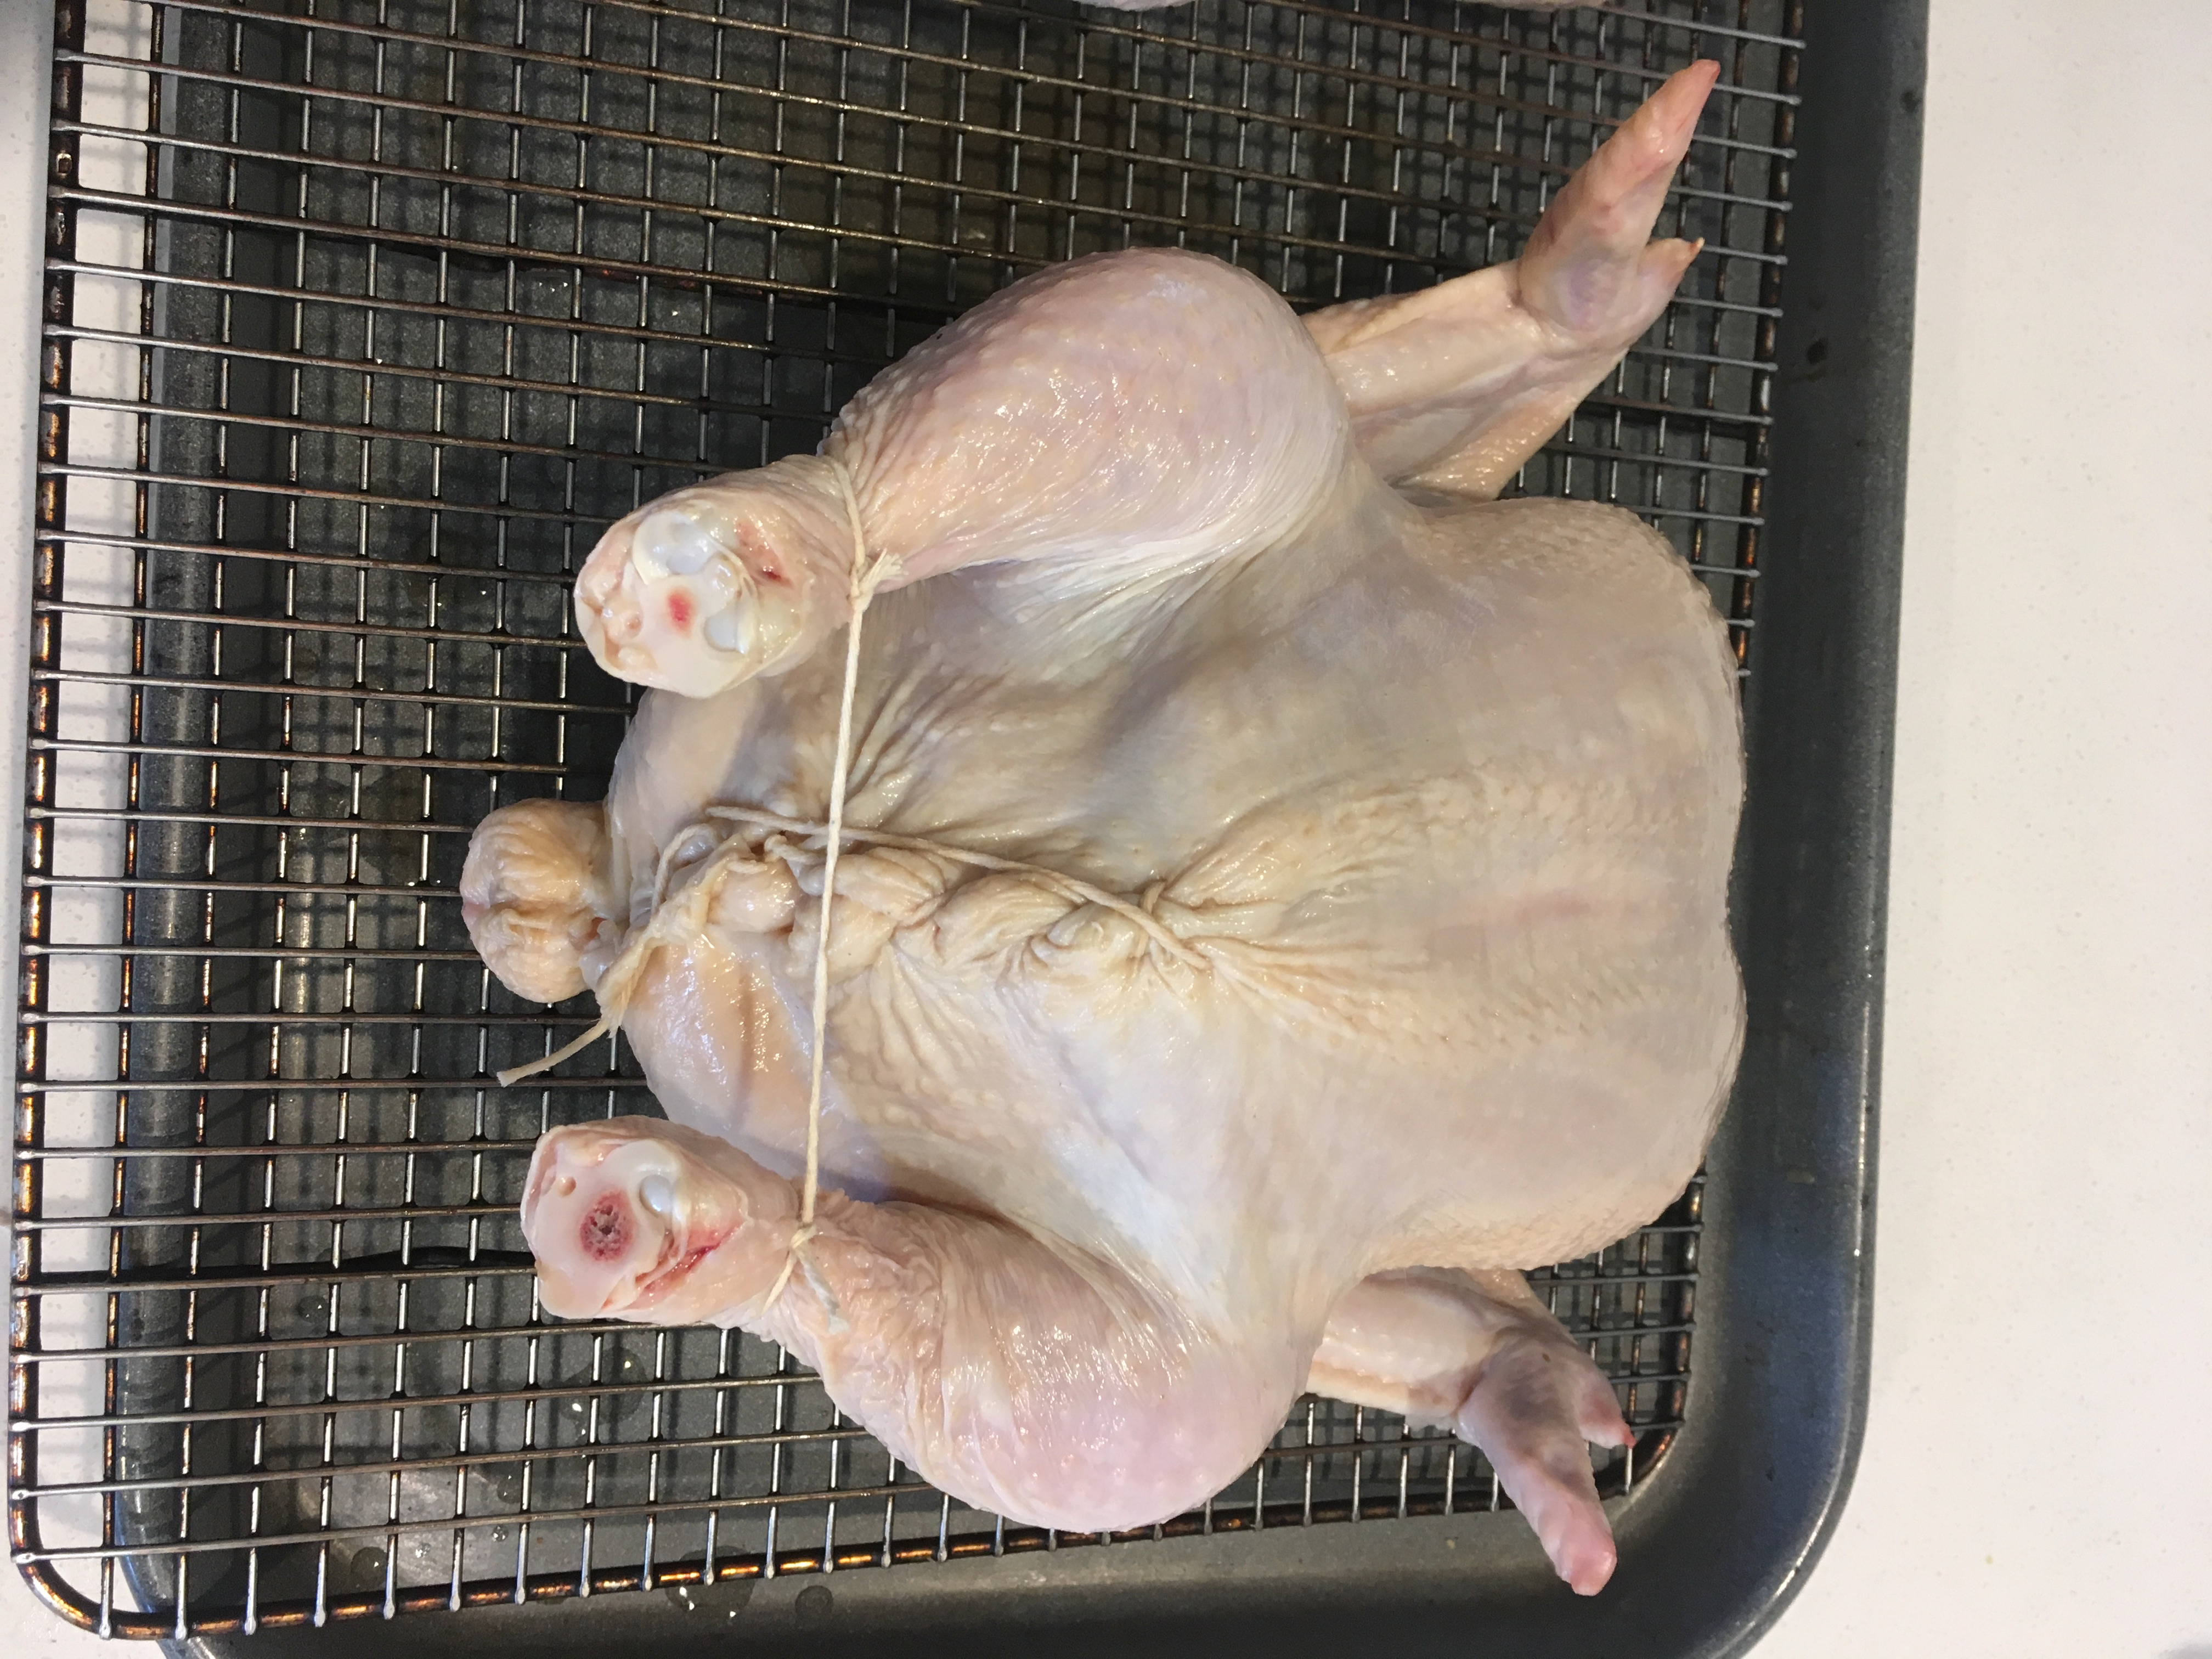
\includegraphics[width=0.25\textwidth]{\imageDir/\fileName/IMG_3219.jpg} \\
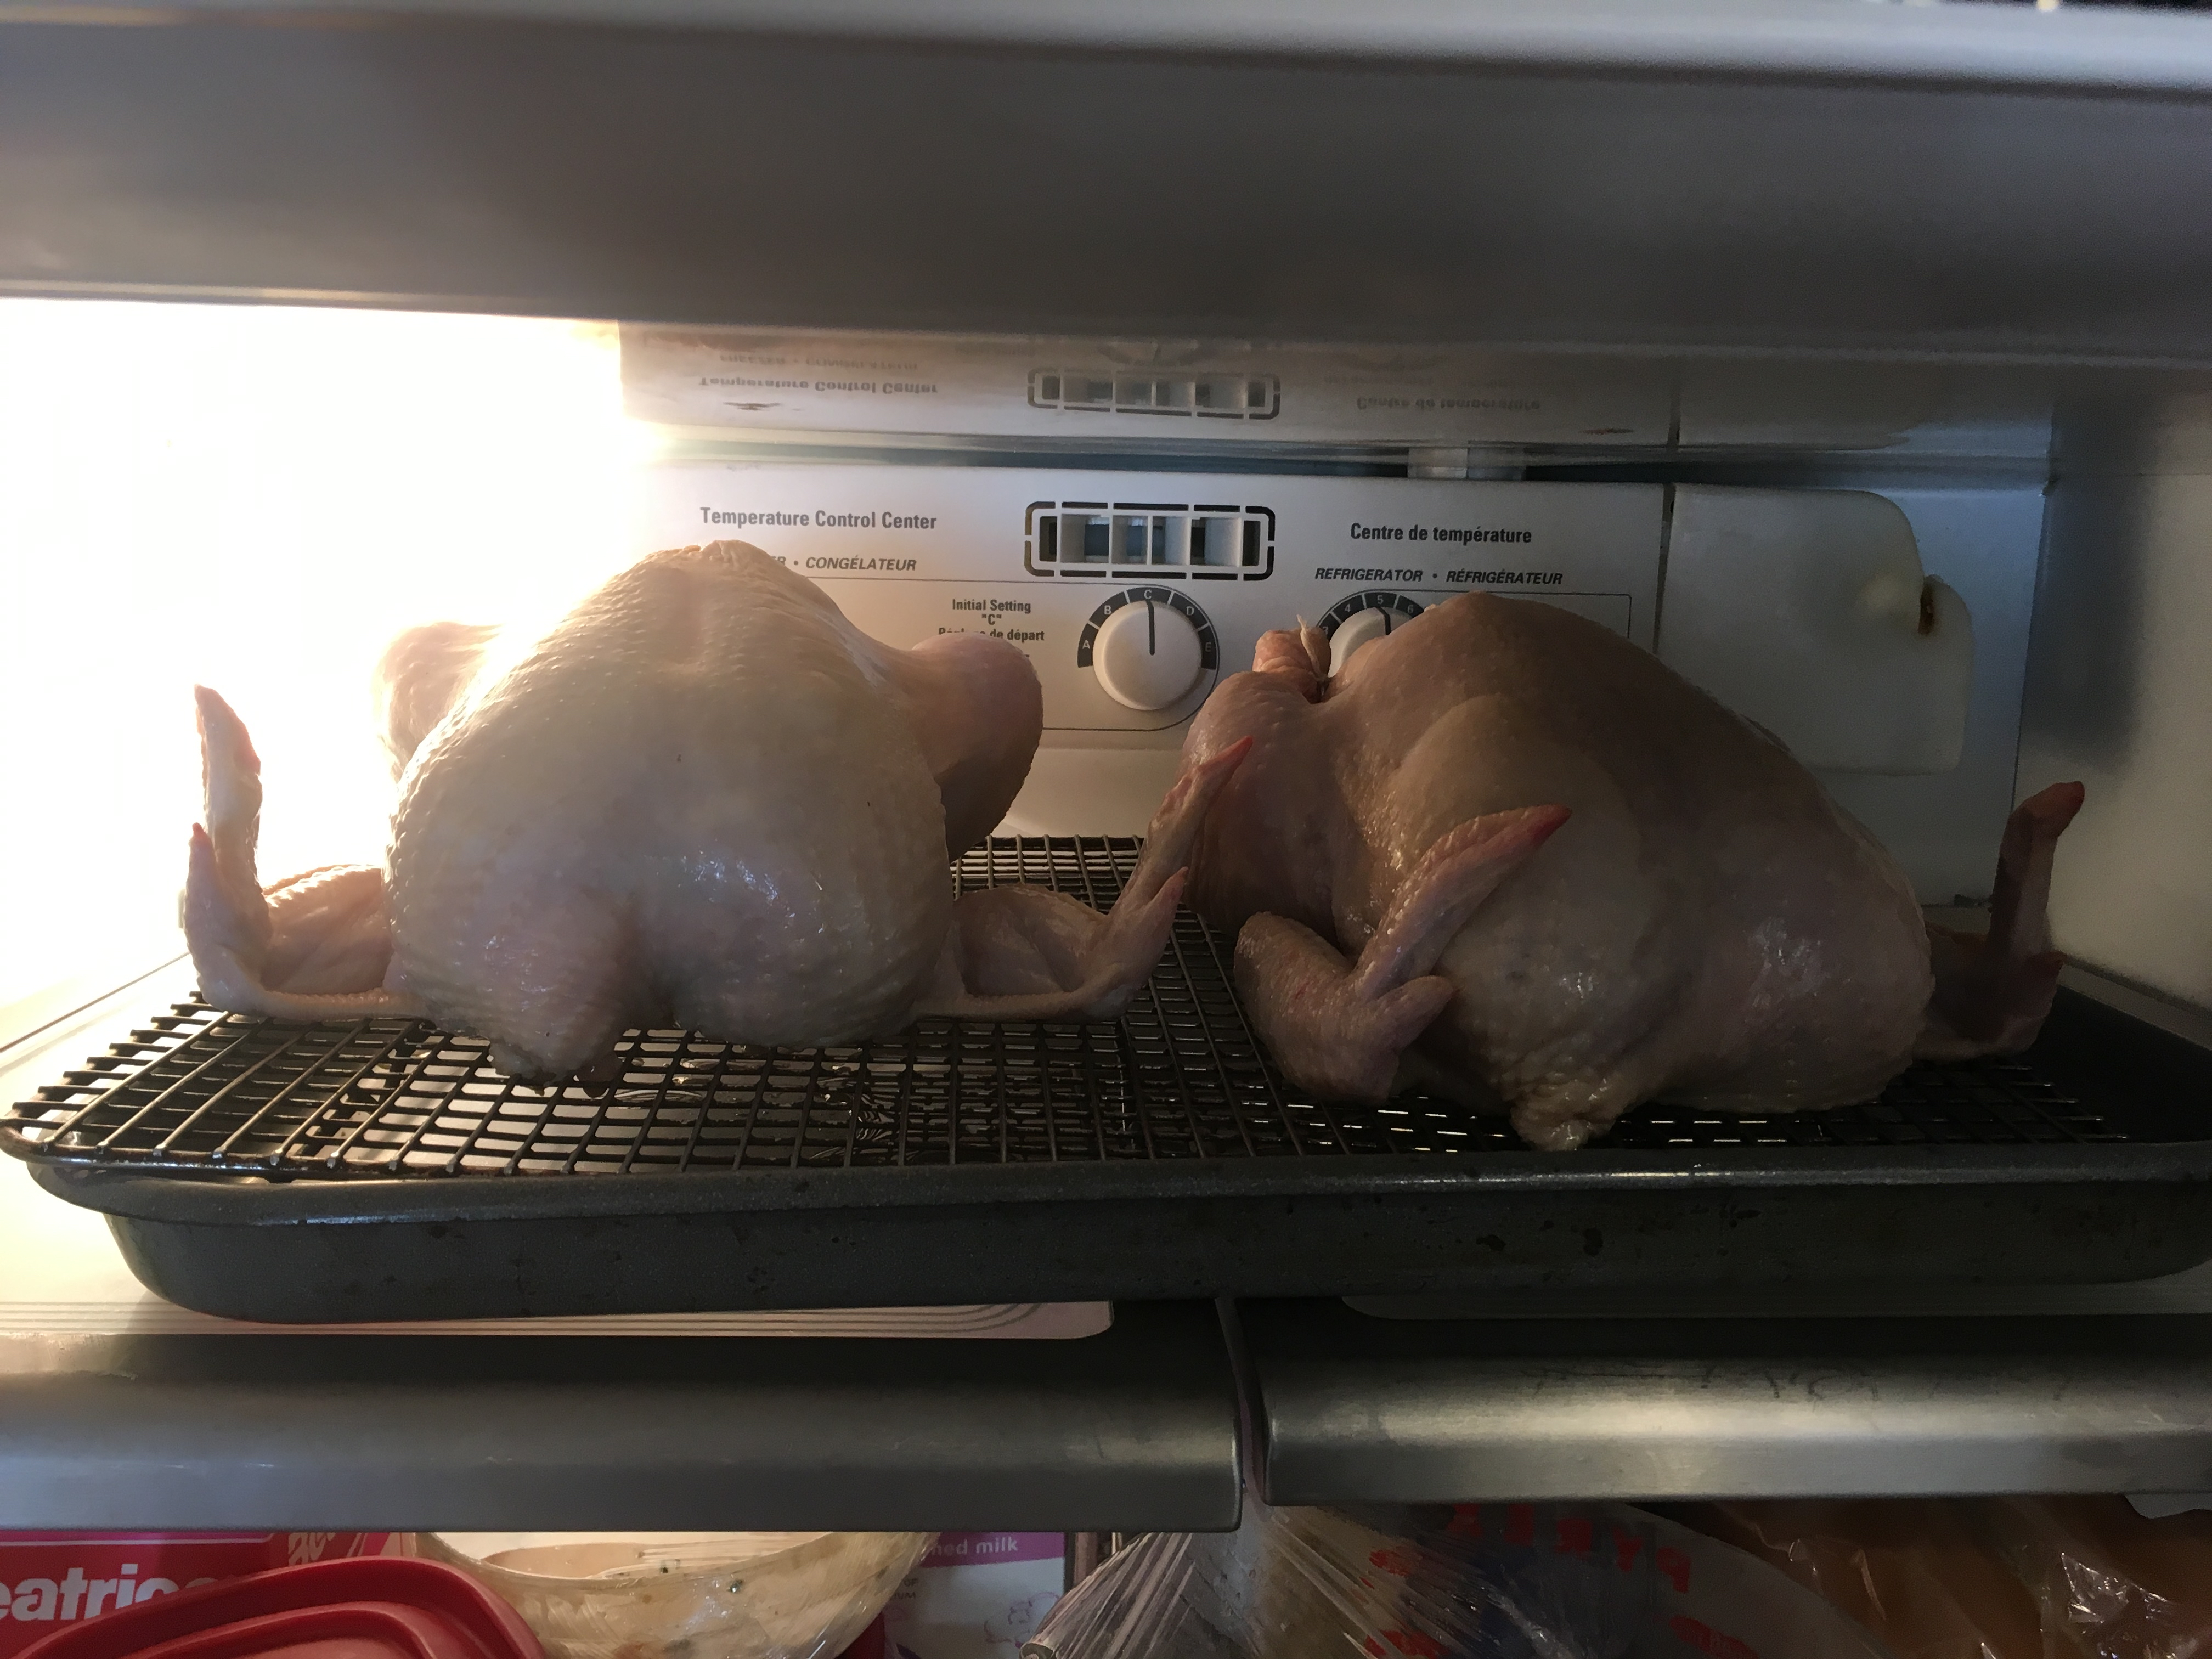
\includegraphics[width=0.25\textwidth]{\imageDir/\fileName/IMG_3220.jpg} &
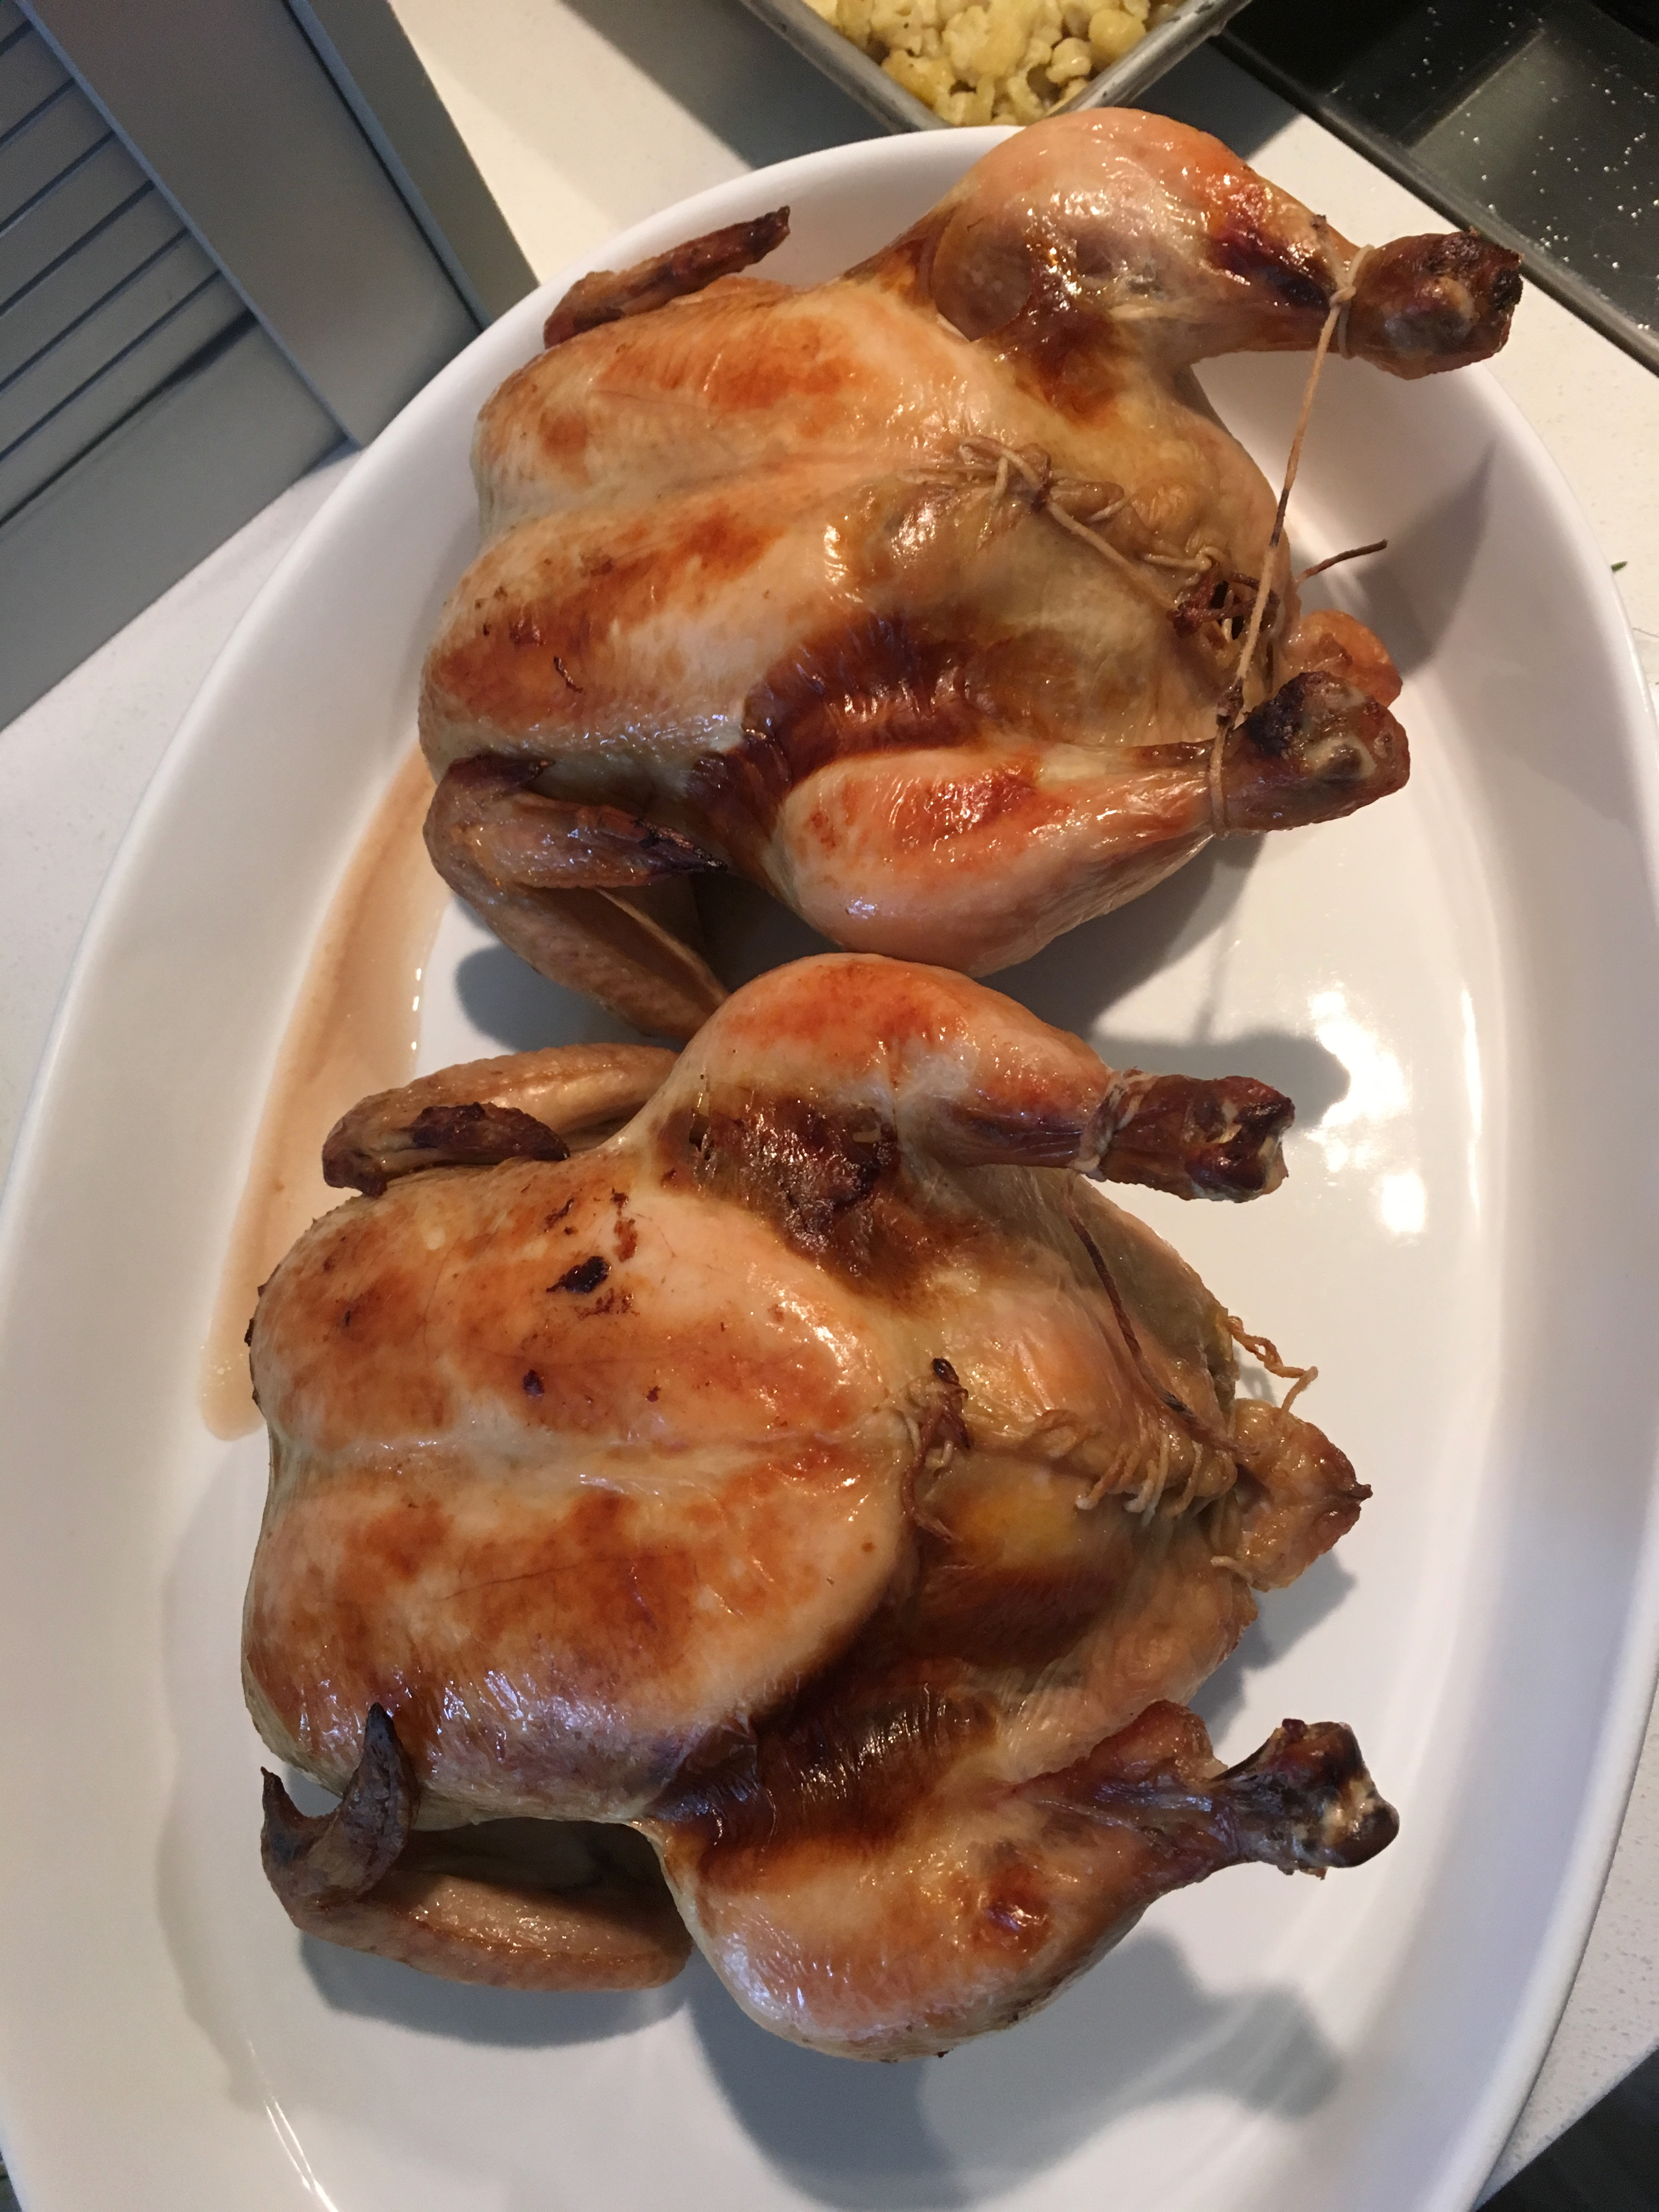
\includegraphics[width=0.25\textwidth]{\imageDir/\fileName/IMG_3228.jpg} \\
\end{tabular}
\end{table}


\end{document}

